\chapter{Najkrótsze ścieżki z jednym źródłem}

W poprzednim rozdziale omówiliśmy prosty algorytm wyszukiwania najkrótszych ścieżek w charakterze przykładu na wykorzystanie w praktyce wcześniej omówionych zagadnień. Doszliśmy do wniosku, że algorytm wykonuje ogromną liczbę operacji, w tym większość z nich niepotrzebnie (jak na przykład próby relaksacji krawędzi, wychodzących z wierzchołków, do których algorytm jeszcze nie potrafił dojść, wykorzystując wcześniej obliczone ścieżki), starając się zminimalizować ilość tych ostatnich, poprzez wprowadzenie dodatkowych warunków do naszej implementacji. Ich obecność pozwalała mieć nadzieję na efektywniejsze działanie algorytmu, jednak asymptotycznie nie uzyskaliśmy żadnej poprawy, nadal oszacowując czas działania algorytmu na ograniczony przez $O \left( V \cdot E \right)$. Nie umknął też naszej uwadze fakt, iż od kolejności wykonywanych relaksacji głównie zależy ilość operacji, jakie algorytm musi wykonać, aby zwrócić poprawny wynik i zakończyć pracę. Nic więc dziwnego, że rozwój algorytmiki zaowocował zaproponowaniem wielu innych rozwiązań tego samego problemu, skupiając się przede wszystkim na wymuszeniu takiej kolejności operacji, aby algorytm wykonywał ich jak najmniej.

\section{Sortowanie topologiczne}

Aby przekonać się o skuteczności takiego podejścia, przedstawimy prosty algorytm \textbf{sortowania topologicznego}, z którego pomocą będziemy mogli odnaleźć wszystkie najkrótsze ścieżki w skierowanym grafie ważonym $G = \left( V, E \right)$ w czasie liniowym (co jest ogromnym skokiem wydajnościowym, jeżeli chodzi o kwadratową złożoność algorytmu Bellmana-Forda)! Niestety, jak się będziemy mieli okazję przekonać, algorytm \textbf{sortowania topologicznego} narzuci nam bardzo silne ograniczenie na postać grafu, dla którego będziemy chcieli dokonywać obliczeń, przez co algorytm ten nie będzie już taki atrakcyjny, jakim wydawał się na początku, jednak będzie nadal wystarczająco skuteczny, by zastosować go w celu wyszukiwania najkrótszych ścieżek.

\textbf{Sortowanie topologiczne} polega na takim posortowaniu wierzchołków, aby dla każdej pary $ \left( v_{i}, v_{j} \right)$, w przypadku istnienia krawędzi pomiędzy tymi wierzchołkami, prowadzącej z $V_{i}$ do $v_{j}$, w posortowanym ciągu $v_{i}$ znajdował się przed wierzchołkiem, do którego dana krawędź prowadzi. Innymi słowy sortowanie topologiczne prowadzi do ustalenia możliwej kolejności odwiedzeń wszystkich wierzchołków w grafie. Jako przykład w literaturze najczęściej można spotkać problem stworzenia listy kolejno wykonywanych czynności na podstawie posiadanego grafu, przedstawiającego zależności między poszczególnymi czynnościami (na przykładzie pieczenia ciasta, bądź kolejności zakładania ubrań). 

Mówiąc o kolejności w grafie oczywistym więc jest, że nie uda nam się ustalić odpowiedniego porządku dla grafów, które będą zawierały cykle, lecz - jak się przekonamy - dla takich danych jesteśmy w stanie ustalić wystarczająco dobry porządek wśród wierzchołków, aby bardzo szybko obliczyć wszystkie najkrótsze ścieżki w zadanym grafie. Poniżej przedstawimy dwie popularne metody wyznaczania takiego porządku, gdzie pierwsza z nich okaże całkowicie bezradna w obliczu wystąpienia cyklu, zaś druga będzie je po prostu ignorować. Należy wyraźnie podkreślić, że w tym drugim przypadku dla grafu zawierającego cykle jako wynik nie otrzymamy porządku topologicznego, lecz uporządkowanie do niego podobne.

\subsection{Algorytm Khana}

Jednym z naturalnych sposobów na wyznaczenie opisanej przez nas kolejności wierzchołków jest rozpoczęcie ich spisywania od tych, do których nie prowadzą żadne krawędzie - powiedzmy, że takie wierzchołki nie mają żadnych "wymagań" by mogły być odwiedzone. Skoro odwiedziliśmy już wszystkie takie wierzchołki, możemy założyć, że pewne "wymagania", które te wierzchołki sobą reprezentują, zostały spełnione i posiadamy nieco większe "możliwości", by czynić zadość "wymaganiom" pozostałych wierzchołków. Takie rozumowanie, przeprowadzone dla wszystkich wierzchołków w grafie bez cykli da nam listę, na którą zostały spisane wierzchołki w porządku topologicznym. Łatwo sobie wyobrazić analogiczne rozumowanie w przypadku wystąpienia cyklu: gdy wierzchołek $v_{A}$ na swojej "liście wymagań" posiada takie, by przed jego odwiedzeniem był odwiedzony węzeł $v_{B}$ (co przedstawilibyśmy na grafie w postaci krawędzi z $v_{B}$ do $v_{A}$), a wierzchołek $v_{B}$ - by przed jego odwiedzeniem był odwiedzony węzeł $v_{A}$. Widzimy, że żadnego z tych warunków nie da się spełnić. Algorytm, opisujący takie działanie, wyglądać mógłby następująco:

\begin{algorithm}[!htbp]
\DontPrintSemicolon
\KwIn{Graf $G = \left( V, E\right)$.}
\KwResult{Lista $O$ z posortowanymi topologicznie wierzchołkami.}
\Begin{
	$ S \longleftarrow $ zbiór wszystkich wierzchołków, do których nie prowadzą żadne krawędzie \;
	$ O \longleftarrow \emptyset $ \;
	\While{$S$ nie jest pusta}{
		Przepnij wierzchołek $v_{i}$ z $S$ na koniec listy $O$ \;
		\ForEach{$e_{ij} : v_{i} \overset{1} \leadsto v_{j}$}{
			Usuń krawędź $e_{ij}$ z grafu $G$ \;
			\If{ do $v_{j}$ nie wchodzą już żadne krawędzie } {
				Wstaw wierzchołek $v_{j}$ do $S$ \;
			}
		}
	}
	\eIf{ w grafie $G$ nadal są wierzchołki }{
		\Return \KwNull \;
	}{
		\Return $O$ \;
	}
}
\caption{ KHAN-TOPOLOGICAL-SORT $\left( G \right)$\label{alg:KhanTopologicalSort}}
\end{algorithm}

Algorytm działa niemal identycznie jak w przeprowadzonym przez nas rozumowaniu. Za punkt wyjścia obieramy listę wierzchołków, do których nie prowadzą żadne krawędzie, a następnie usuwamy wszystkie te, które wychodzą od wierzchołków, które już odwiedziliśmy. W momencie, gdy do jakiegoś węzła przestają prowadzić krawędzie w grafie, dodajemy go do listy węzłów, które sekwencyjnie odwiedzamy. Jest to sytuacja równoważna ze spełnieniem wszystkich "wymagań", by dany wierzchołek móc odwiedzić. To co może okazać się problematyczne to zdobycie informacji na temat ilości krawędzi, wchodzących do każdego pojedynczego wierzchołka, gdyż - jak pamiętamy - zdecydowaliśmy się na przedstawienie struktury połączeń w grafie za pomocą list sąsiedztwa, które nam takiej wiedzy nie dają. Jest on jednak bardzo prosty do rozwiązania, gdyż aby takie informacje zdobyć musimy przejść po wszystkich krawędziach w grafie, gromadząc w osobnej tablicy $deg \left[1 \cdots \left| V \right| \right]$ informację o liczbie łuków, wchodzących do poszczególnych węzłów o identyfikatorach z zakresu od $1$ do $\left| V \right|$ (przy czym nie interesuje nas nic poza ich liczebnością). Czas, jaki potrzebujemy na jednorazowe przejście po wszystkich krawędziach grafu $G$ jest oczywiście liniowa i wynosi $O \left( \left| E \right| \right) $. Następnie ta tablica posłuży nam do symulowania takich wydarzeń jak: usunięcie krawędzi z grafu, sprawdzenie, czy do danego wierzchołka przestały prowadzić jakiekolwiek łuki. Nie usuwając krawędzi z grafu zaraz po przejściu przez nie, a jedynie symulując ich usunięcia narażamy się na sytuacje, w których algorytm zacznie nieprzerwanie krążyć pomiędzy węzłami w grafie, które tworzą cykl - sprawdzenie, czy taki występuje następuje dopiero pod sam koniec algorytmu w wierszach 9-12. Możemy sobie jednak z tym problemem poradzić równie łatwo, co z wyznaczaniem ilości węzłów wchodzących do grafu . Jedyne, co musimy zauważyć to fakt, że z każdym powtórzeniem instrukcji 3-8 dodajemy do zbioru $S$ kolejny wierzchołek grafu. W przypadku natrafienia na cykl i nieusuwania krawędzi każde wejście do węzła $v_{i}$ po ścieżce, należącej do cyklu, spowoduje, że zmniejszymy wartość licznika $deg \left[ i \right]$ o jeden (symulując tym samym usunięcie krawędzi). Jeżeli okaże się, że po pierwszym przejściu taką ścieżką $deg \left[ i \right] = 0 $ (co odpowiada braku krawędzi wchodzących do $v_{i}$) dla każdego węzła, należącego do cyklu to wpadniemy z nieskończoną pętlę, dodając do zbioru $S$ kolejne węzły, a następnie te same węzły usuwając w kroku 4. Jednym z wielu pomysłów na rozwiązanie tego problemu jest wprowadzenie ograniczenia na ilość elementów listy $O$ - dla poprawnie wykonanego algorytmu będzie ona zawsze długości $ \left| V \right| $, podczas gdy dla omawianego przypadku złego zachowania się algorytmu bardzo szybko liczba tych elementów przekroczy ich oczekiwaną ilość.


\begin{figure}[!htbp]
	\centering
	\begin{subfigure}[b]{0.25\textwidth}
		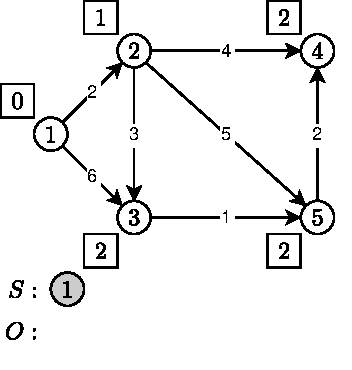
\includegraphics[width=\textwidth]{Chapter_II/KHAN-TOPOLOGICAL-SORT-Example/a.pdf}
		\caption{}
	\end{subfigure}%
	\qquad
	\begin{subfigure}[b]{0.25\textwidth}
		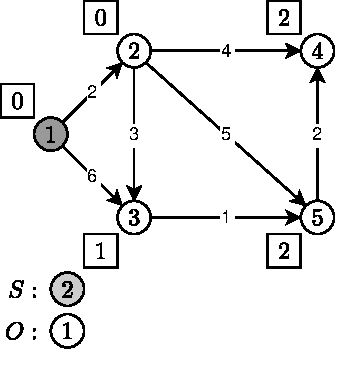
\includegraphics[width=\textwidth]{Chapter_II/KHAN-TOPOLOGICAL-SORT-Example/b.pdf}
		\caption{}
	\end{subfigure}
	\qquad
	\begin{subfigure}[b]{0.25\textwidth}
		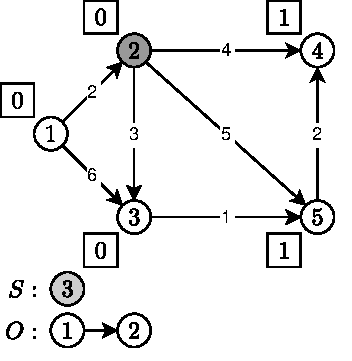
\includegraphics[width=\textwidth]{Chapter_II/KHAN-TOPOLOGICAL-SORT-Example/c.pdf}
		\caption{}
	\end{subfigure}
	\begin{subfigure}[b]{0.25\textwidth}
		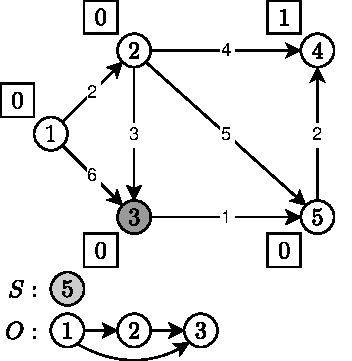
\includegraphics[width=\textwidth]{Chapter_II/KHAN-TOPOLOGICAL-SORT-Example/d.pdf}
		\caption{}
	\end{subfigure}%
	\qquad
	\begin{subfigure}[b]{0.25\textwidth}
		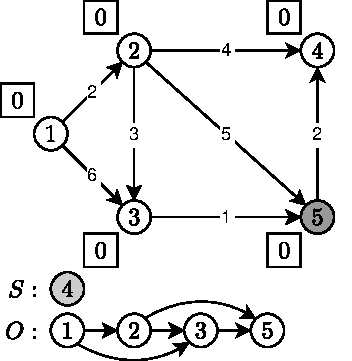
\includegraphics[width=\textwidth]{Chapter_II/KHAN-TOPOLOGICAL-SORT-Example/e.pdf}
		\caption{}
	\end{subfigure}
	\qquad
	\begin{subfigure}[b]{0.25\textwidth}
		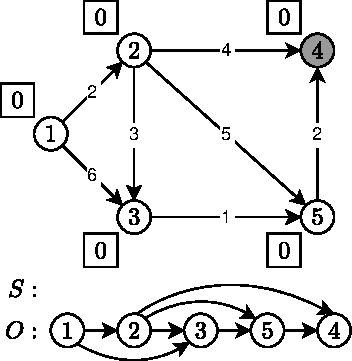
\includegraphics[width=\textwidth]{Chapter_II/KHAN-TOPOLOGICAL-SORT-Example/f.pdf}
		\caption{}
	\end{subfigure}
	\caption{\textbf{Działanie algorytmu Khana} \textbf{(a)} Sytuacja początkowa algorytmu. Na liście $S$ znajdują się wszystkie węzły, do których - przed rozpoczęciem działania algorytmu - nie wchodziły żadne krawędzie. W kwadratach przy każdym z węzłów znajduje się liczba takich krawędzi $e \in E$, które wchodzą do danego wierzchołka - reprezentują one elementy tablicy $deg \left[ i \right]$, gdzie $i$ to identyfikator węzła, przy którym znajduje się dany element. \textbf{(b)} Algorytm wybiera z listy $S$ jedyny możliwy element i usuwa z grafu wszystkie krawędzie, wychodzące z wybranego węzła, dodając jednocześnie do listy $O$ każdy węzeł, do którego, w wyniku usunięcia tych krawędzi, nie prowadzi już żaden łuk. Usuwanie połączenia $v_{i} \overset{1} \leadsto v_{j}$ symbolizujemy zmniejszeniem wartości elementu $deg \left[ j \right]$. \textbf{(c)} Usunięcie krawędzi wychodzących z następnego, pobranego z listy $S$, elementu spowodowało dodanie do listy $S$ węzła $v_{3}$. Badany element $v_{2}$ - podobnie jak w poprzednim przypadku - po wyciągnięciu z listy $S$ przepinamy do listy $O$. \textbf{(d)} Dodanie do listy $S$ węzła $v_{5}$ przy usuwaniu wszystkich krawędzi $e \in \left\{ e_{ij} : i = 3 \right\}$ i przepięcie badanego elementu $v_{3}$ na listę $O$. \textbf{(e)} Wykonanie kolejnej pętli algorytmu i dodanie skanowanego elementu $v_{5}$ do listy wynikowej.  \textbf{(f)} Ostatni krok algorytmu. Zauważmy, że w grafie nie ma już żadnych łuków (wszystkie elementy z tablicy $deg$ zostały wyzerowane), więc algorytm zakończył się poprawnie, a badana sortowana sieć nie miała cykli.} \label{fig:exampleKhan}
\end{figure}

Czas działania takiej metody jest oczywiście liniowy, zależny od ilości zarówno węzłów jak i krawędzi w grafie. Zależnie od tego, czy w węzłach przechowujemy informację o liczbie wchodzących do nich krawędzi, te pierwsze będziemy musieli przejrzeć w czasie $O \left( \left| V \right| \right)$ w poszukiwaniu takich węzłów, które takowych krawędzi nie mają, zaś jeżeli takich informacji nie mamy - wówczas będziemy musieli je sami wygenerować, skanując wszystkie krawędzie w grafie (co zajmie nam $O \left( \left| E \right| \right)$ czasu). Bez względu na wcześniej wykonany krok, właściwa część algorytmu polega na usunięciu wszystkich krawędzi z grafu (gdyż taki chcemy uzyskać rezultat dla prawidłowej sieci) w czasie $O \left( \left| E \right| \right)$.

\subsection{Przeszukiwanie w głąb}

Alternatywnym sposobem na topologiczne uporządkowanie grafów w sieci jest wykorzystanie właściwości, posiadanych przez prosty algorytm przeszukiwania w głąb, w skrócie \textsf{DFS} (ang. \textit{Depth-First Search}). Aby posortować topologicznie wszystkie węzły w gafie $G = \left( V, E \right)$ wykorzystujemy fakt, że wspomniany algorytm oznacza dany węzeł $V$ jako przetworzony dopiero w momencie, gdy wszystkie węzły, do których jest w stanie dojść z badanego węzła, są oznaczone. Innymi słowy nie jest możliwa sytuacja, by w grafie został oznaczony węzeł, którego wszystkie dzieci (a także jego dalsi potomkowie) nie zostały oznaczone. Zapisując kolejność takich operacji (oznaczania węzłów jako przetworzone), a następnie odtwarzając ją w kolejności odwrotnej uzyskujemy listę z poprawnie posortowanymi topologicznie węzłami (odwrotna sytuacja do przedstawionej wcześniej ma następującą interpretacje: żaden węzeł $v_{i}$ nie zostanie zaznaczony, gdy istnieje jakikolwiek węzeł $v_{j}$, który jest jeszcze nie zaznaczony, a który posiada krawędź $v_{j} \overset{1} \leadsto v_{i}$).

\begin{algorithm}[!htbp]
\DontPrintSemicolon
\KwIn{Graf $G = \left( V, E\right)$.}
\KwResult{Lista $O$ z posortowanymi topologicznie wierzchołkami.}
\Begin{
	Wykonaj \textsf{DFS} dla grafu wejściowego $G$ \;
	Wstaw na początek listy $O$ każdy wierzchołek $V$, kiedy ten tylko zostanie oznaczony jako przetworzony. \;
	\Return $O$ \;
}
\caption{ BFS-TOPOLOGICAL-SORT $\left( G \right)$\label{alg:BFSTopologicalSort}}
\end{algorithm}

W algorytmie od razu niejawnie dokonujemy odwrócenia elementów, które znajdują się na liście $O$ poprzez wstawianie każdego wierzchołka na początek tej listy, nie na jej koniec. Algorytm oczywiście działa w czasie liniowym, podobnie jak sam \textsf{DFS} ($ \Theta \left( \left| V \right| + \left| E \right| \right)$). Wspomnieliśmy na początku rozdziału, poświęconemu sortowaniom topologicznym grafów, że drugi z omawianych algorytmów posiada nad pierwszym tę przewagę, że nie przerywa pracy nawet w momencie napotkania cyklu. Nie jest to do końca prawdą, gdyż zachowanie się algorytmu \textsf{DFS} głównie zależy od intencji jego autora, lecz możemy napisać go w taki sposób, aby przeglądając graf wgłąb, po natrafieniu na już odwiedzony wierzchołek kontynuował swoją pracę (to jest albo wycofał się z aktualnie badanego wierzchołka, zaznaczając go jako przetworzony, albo - w przypadku, gdy pozostałe krawędzie badanego węzła prowadzą do jeszcze nieodwiedzonych węzłów - kontynuował przeszukiwanie wgłąb). Innymi słowy - możemy go zmusić by ignorował cykle, występujące w badanym grafie.

\begin{figure}[!htbp]
	\centering
	\begin{subfigure}[b]{0.2\textwidth}
		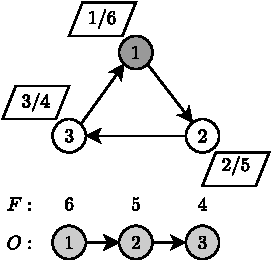
\includegraphics[width=\textwidth]{Chapter_II/BFS-TOPOLOGICAL-SORT-Example/a.pdf}
		\caption{}
	\end{subfigure}%
	\qquad \qquad
	\begin{subfigure}[b]{0.18\textwidth}
		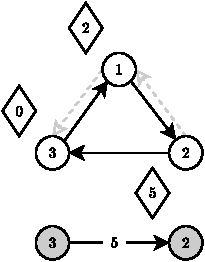
\includegraphics[width=\textwidth]{Chapter_II/BFS-TOPOLOGICAL-SORT-Example/b.pdf}
		\caption{}
	\end{subfigure}
	\qquad \qquad
	\begin{subfigure}[b]{0.18\textwidth}
		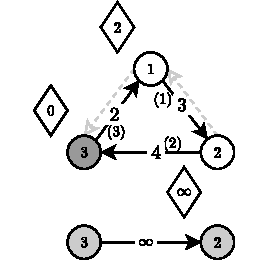
\includegraphics[width=\textwidth]{Chapter_II/BFS-TOPOLOGICAL-SORT-Example/c.pdf}
		\caption{}
	\end{subfigure}
	\caption{\textbf{Przykład złego działania \textsf{DFS} dla grafu z cyklem} \textbf{(a)} Graf po wykonaniu algorytmu \textsf{DFS}. W rombach znajdują się charakterystyczne dla grafu wartości w postaci $x/y$, gdzie $x$ oznacza czas odwiedzenia danego węzła, zaś $y$ to czas jego przetworzenia (po przetworzeniu wszystkich jego dzieci i ich potomków oraz wycofaniu się z niego). Lista $O$ zawiera "poprawnie" uporządkowane węzły, w kolejności malejącej względem czasu przetwarzania węzłów. Algorytm rozpoczyna pracę od pierwszego węzła w grafie. \textbf{(b)} Poprawnie wykonany algorytm wyszukiwania najkrótszej ścieżki $v_{3} \overset{1} \leadsto v_{2}$. $c \left( 3, 2 \right) = \delta \left( 3, 2 \right) = 5$. \textbf{(c)} Błędne rozwiązanie dla algorytmu opartego o listę $O$ z rysunku pierwszego. Cyfry w nawiasach oznaczają kolejność wykonywania relaksacji, wynikającej z uporządkowania węzłów na liście $O$.} \label{fig:exampleDFS}
\end{figure}

Niestety - tak wygenerowany porządek nie nadaje się do wykorzystania w algorytmie wyszukiwania najkrótszych ścieżek, który działałby w czasie liniowym. Choć początkowo może się wydawać, że ignorowanie cykli nie szkodzi, a wręcz jest po naszej myśli (algorytm \textsf{DFS}, napotykając ścieżkę zamykającą cykl, nie zdecyduje się na pójście tą ścieżką, podobnie jak relaksacja takiej ścieżki nigdy nie przyniesie żadnego rezultatu - innymi słowy jest zbędna), lecz prosty przykład wystarcza, by algorytm wyszukiwania najkrótszych ścieżek, który opiera się o sortowanie topologiczne, zwracał nam niepoprawne wyniki.

\subsection{Sortowanie topologiczne}

Jak widzimy z powyższych przykładów, możliwości wykorzystania sortowania topologicznego w algorytmach wyszukiwania najkrótszych ścieżek są ograniczone jedynie do małej klasy grafów - stanowczo za małej, jeżeli chodzi o grafy, reprezentujące rzeczywiste sieci drogowe. Istnieją jednak pewne problemy (mniej trywialne od pieczenia ciasta, czy kolejności nakładania ubrań), w których taki algorytm się przydaje i jest chętnie stosowany głównie ze względu na swoją szybkość działania - liniową, proporcjonalnie do ilości krawędzi w grafie. Implementacja algorytmu sprowadza się do wykonania relaksacji dla każdej krawędzi, wychodzących z węzłów posortowanych topologicznie, w której to kolejności powinniśmy postępować.

\begin{algorithm}[!htbp]
\DontPrintSemicolon
\Begin{
	\ForEach{ $v_{i}$ w porządku topologicznym } {
		\ForEach{$e_{ij} : v_{i} \overset{1} \leadsto v_{j}$}{
			$RELAX \left( v_{i}, v_{j} \right)$ \;
		}
	}
}
\caption{ TOPOLOGICAL-SHORTEST-PATH $\left( G \right)$\label{alg:topologicalShorestPath}}
\end{algorithm}

Aby udowodnić poprawność działania takiego algorytmu, odwołamy się do dwóch, wcześniej przedstawionych (w rozdziale \ref{sub:shortestPathProperties}), lematów: mówiącym o optymalnej podstrukturze grafu (\ref{lem:optimalSubstructure}) oraz o własności zbieżności dla najkrótszych ścieżek (\ref{lem:convergenceProperty}).

\begin{proof}
Załóżmy indukcyjnie, że algorytm przeskanował już wierzchołki $v_{i} : i \in \left\{ 1, 2, \cdots, k \right\}$ i dla każdego z nich ich waga jest optymalna ($d \left( i \right) = \delta \left( s, v_{i} \right)$). W oczywisty sposób pierwszy krok indukcyjny jest spełniony: dla $k = 1$ naszym jedynym wierzchołkiem, który został obsłużony jest wierzchołek początkowy - źródło, którego $d \left( s \right) = \delta \left( s, s \right) = 0$. Przyjrzyjmy się teraz sytuacji, w której algorytm bada węzeł $k+1$'y (a nie konkretnie $v_{k+1}$). Niech najkrótszą ścieżką do tego węzła będzie $P = \left \langle v_{1}, v_{2}, \ldots, v_{h}, k+1 \right \rangle $. Z lematu \ref{lem:optimalSubstructure} (o optymalnej podstrukturze) wiemy, każda podścieżka ścieżki $P$ jest najkrótszą ścieżką, w szczególności jest nią ścieżka $P^{'} = \left \langle v_{1}, v_{2}, \ldots, v_{h} \right \rangle $. Z faktu, że wszystkie wierzchołki w grafie są posortowane topologicznie oraz, że krawędź $v_{h} \overset{1}\leadsto k+1 \in E$ (co nam gwarantuje istnienie ścieżki $P$) wynika, że wierzchołek $v_{h}$ jest węzłem, dla którego $h \in \left\{ 1, 2, \cdots, k \right\}$ w związku z czym, na mocy założenia indukcyjnego, wartość $v_{h}.d = \delta \left( s, v_{h} \right)$. Zgodnie z lematem \ref{lem:convergenceProperty}, jeżeli w dowolnym momencie przed relaksacją krawędzi $v_{h} \overset{1}\leadsto k+1$ wartość $v_{h}.d = \delta \left( s, v_{h} \right)$ to po relaksacji tej krawędzi już zawsze $ \left( k+1 \right).d = \delta \left( s, v_{h} \right) $ (jest optymalna). Z faktu istnienia takiej krawędzi oraz z uporządkowania topologicznego wszystkich węzłów w grafie wiemy, że waga, trzymana przez wierzchołek $v_{h}$ zawsze będzie optymalna przed przystąpieniem do przechodzenia po krawędzi $v_{h} \overset{1}\leadsto k+1$, co kończy dowód.
\end{proof}


\begin{figure}[!htbp]
	\centering
	\begin{subfigure}[b]{0.18\textwidth}
		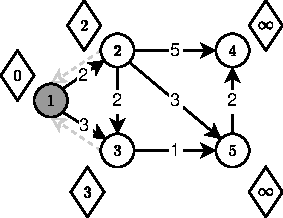
\includegraphics[width=\textwidth]{Chapter_II/TOPOLOGIC-SHORTEST-PATH-Example/a.pdf}
		\caption{}
	\end{subfigure}
	\begin{subfigure}[b]{0.18\textwidth}
		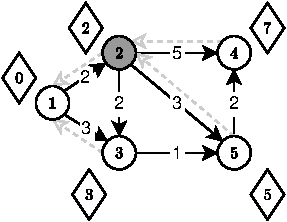
\includegraphics[width=\textwidth]{Chapter_II/TOPOLOGIC-SHORTEST-PATH-Example/b.pdf}
		\caption{}
	\end{subfigure}
	\begin{subfigure}[b]{0.18\textwidth}
		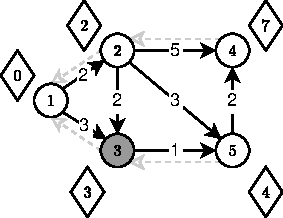
\includegraphics[width=\textwidth]{Chapter_II/TOPOLOGIC-SHORTEST-PATH-Example/c.pdf}
		\caption{}
	\end{subfigure}
	\begin{subfigure}[b]{0.18\textwidth}
		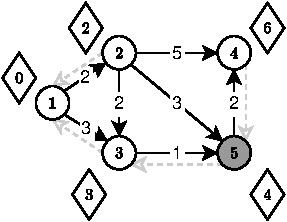
\includegraphics[width=\textwidth]{Chapter_II/TOPOLOGIC-SHORTEST-PATH-Example/d.pdf}
		\caption{}
	\end{subfigure}
	\begin{subfigure}[b]{0.18\textwidth}
		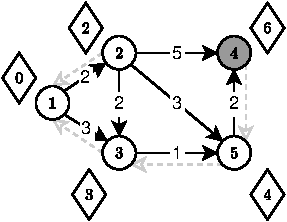
\includegraphics[width=\textwidth]{Chapter_II/TOPOLOGIC-SHORTEST-PATH-Example/e.pdf}
		\caption{}
	\end{subfigure}
	\caption{\textbf{Przykład dla ustalonego porządku topologicznego węzłów: $v_{1}, v_{2}, v_{3}, v_{5}, v_{4}$.}} \label{fig:exampleTopologicalShotrestPath}
\end{figure}

\newpage
\section{Generyczny algorytm Dijkstry}

Pokazaliśmy w poprzednich rozdziałach, że kolejność przetwarzania węzłów może mieć ogromny wpływ na szybkość działania algorytmu - od przeglądania wierzchołków w kolejności narzuconej nam przez ich uporządkowanie w strukturach grafu (w czasie $ O \left( \left| V \right| \cdot \left| E \right| \right)$), aż do badania wierzchołków w porządku topologicznym ($ O \left( \left| V \right| + \left| E \right| \right)$). Oba te algorytmy miały zasadnicze wady: albo działały w czasie dużo poniżej naszych oczekiwań, wykonując zatrważającą ilość niepotrzebnych operacji, albo nie nadawały się do użytku w sieciach, które my chcemy badać (z nieujemnymi cyklami). W tym rozdziale przedstawimy kolejny sposób przeglądania wierzchołków grafu $G = \left( V, E \right)$, pokażemy generyczny algorytm na nim oparty, a także udowodnimy jego poprawność. Bazując na kontrprzykładzie, wykażemy także, że nie działa on dla grafów, które zawierają krawędzie o ujemnych wagach (a co za tym idzie dla grafów z ujemnymi cyklami). Algorytm, opracowany przez holenderskiego informatyka Edsgera Dijkstrę, okaże się podstawą do powstania szeregu jego modyfikacji, którym niejednokrotnie zawdzięcza asymptotycznie szybsze czasy działania, a które omówimy w tym rozdziale, skupiając się na ich własnościach.

\subsection{Algorytm Dijkstry}

Sama idea algorytmu jest bardzo podobna do poprzedniej tj. zakłada wykonywanie relaksacji dla wszystkich krawędzi aktualnie badanych wierzchołków, których to kolejność jest w specyficzny sposób ustalana. W przypadku algorytmu opartego na sortowaniu topologicznym grafu był to właśnie ten porządek, który zapewniało nam sortowanie. W Przypadku algorytmu Dijkstry mamy regułę, która mówi, że wierzchołki są skanowane w niemalejącej kolejności ich etykiet (atrybutów $d$ - odległości węzła od źródła $s$), co wiąże się z wykorzystaniem w naszym algorytmie \textbf{kolejek priorytetowych}, które zapewniają nam właśnie taki porządek. Jak się później okaże - omawiane modyfikacje algorytmu Dijkstry różnią się głównie jej implementacją.

Aby wprowadzić nieco formalizmu przyjmiemy, że mamy dwa zbiory rozłączne: $S$, który na początku działania algorytmu jest pusty - do niego trafiać będą przetworzone już wierzchołki - oraz $\overline{s}$, w którym na początku przechowywane są wszystkie węzły. Jak już wspomnieliśmy, algorytm ma za zadanie sekwencyjne pobierać ze zbioru $\overline{S}$ takie wierzchołki $v_{i}$, by $v_{i}.d = \min \left\{ v_{j}.d : v_{j} \in \overline{S} \right\}$, przenosić je do zbioru wierzchołków $S$ oraz wykonywać relaksacje dla każdej krawędzi, która wychodzi z tego wierzchołka. Oczywiście - tak jak w każdym poprzednim algorytmie - na początku inicjalizujemy graf metodą \textsc{INIT-GRAPH} $\left( G, s \right)$. Pseudokod generycznego algorytmu Dijkstry wygląda tak, jak przedstawiono poniżej.

\begin{algorithm}[!htbp]
\DontPrintSemicolon
\Begin{
	$S \longleftarrow \emptyset $ \;
	$\overline{S} \longleftarrow \left\{ v : v \in V \right\} $ \;
	\While{$\overline{S}$ nie jest pusty} {
		$v \longleftarrow  v_{i} : v_{i}.d = \min \left\{ v_{j}.d : v_{j} \in \overline{S} \right\}$ \;
		$S \longleftarrow S \cup \left\{ v \right\}$ \;
		$\overline{S} \longleftarrow \overline{S} - \left\{ v \right\}$ \;
		\ForEach{$e_{ij} : v_{i} \overset{1} \leadsto v_{j}$}{
			$RELAX \left( v_{i}, v_{j} \right)$ \;
		}
	}
}
\caption{ GENERIC-DIJKSTRA $\left( G, s \right)$\label{alg:GenericDijksta}}
\end{algorithm}

gdzie w prawdziwej implementacji linijki $5-7$ zwykle zastępuje się operacją $\textrm{\textsc{EXTRACT-MIN}} \left( Q \right)$, gdzie $Q$ to nasza kolejka priorytetowa. Zbioru $S$ zaś w ogóle się nie uwzględnia, gdyż służy on tylko do celów przeprowadzenia dowodów poprawności tego algorytmu i wykazania, że jest on poprawnie skonstruowany (niezmiennikiem pętli $4-9$ w tym przypadku będzie $Q = V - S$). Odnajdywaniem najmniejszego elementu (w sensie dystansu wierzchołka do źródła) i usuwaniem go ze zbioru $\overline{S}$ zajmuje się, wymieniona wyżej, operacja (wtedy $\overline{S} = Q$). Na przykładzie \ref{fig:exapleDijkstraDLList} jako kolejkę priorytetową wykorzystano podwójnie wiązaną listę (która oczywiście nie jest najfortunniejszym wyborem), której czas, potrzebny na wyciągnięcie z niej najmniejszego elementu, jest zależny od ilości tych elementów na liście (w najgorszym przypadku $ \left| V \right| $.

\begin{figure}[!h]
	\centering
	\begin{subfigure}[b]{0.3\textwidth}
		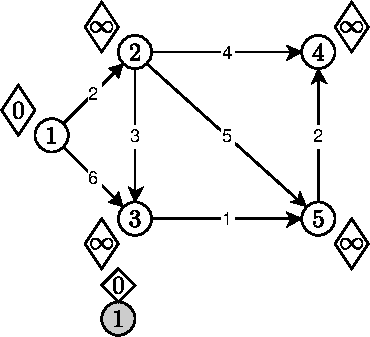
\includegraphics[width=\textwidth]{Chapter_II/DIJKSTRA-DLList/a.pdf}
		\caption{}
	\end{subfigure}%
	\begin{subfigure}[b]{0.3\textwidth}
		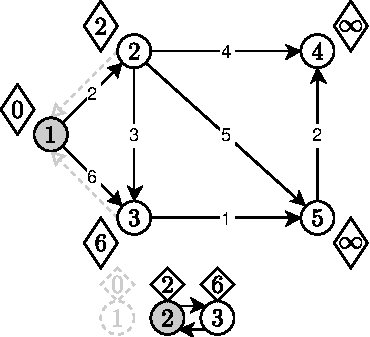
\includegraphics[width=\textwidth]{Chapter_II/DIJKSTRA-DLList/b.pdf}
		\caption{}
	\end{subfigure}
	\begin{subfigure}[b]{0.3\textwidth}
		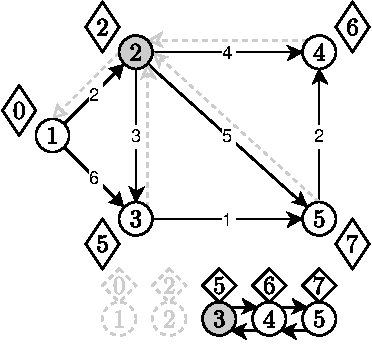
\includegraphics[width=\textwidth]{Chapter_II/DIJKSTRA-DLList/c.pdf}
		\caption{}
	\end{subfigure}
	\begin{subfigure}[b]{0.3\textwidth}
		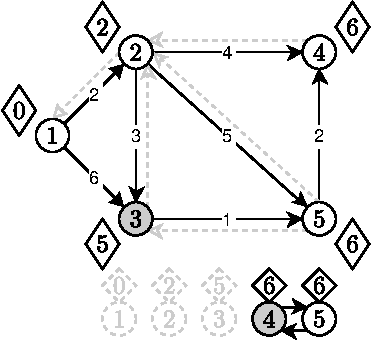
\includegraphics[width=\textwidth]{Chapter_II/DIJKSTRA-DLList/d.pdf}
		\caption{}
	\end{subfigure}%
	\begin{subfigure}[b]{0.3\textwidth}
		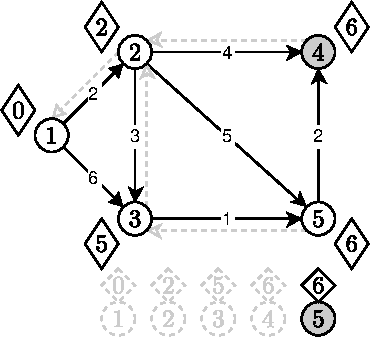
\includegraphics[width=\textwidth]{Chapter_II/DIJKSTRA-DLList/e.pdf}
		\caption{}
	\end{subfigure}
	\begin{subfigure}[b]{0.3\textwidth}
		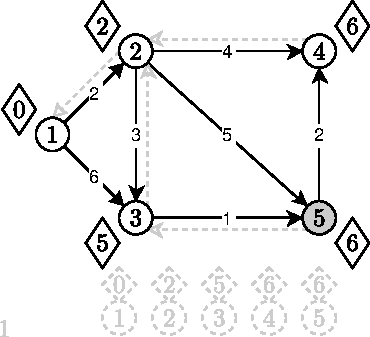
\includegraphics[width=\textwidth]{Chapter_II/DIJKSTRA-DLList/f.pdf}
		\caption{}
	\end{subfigure}
	\caption{\textbf{Działanie algorytmu Dijkstry} \textbf{(a)} Sytuacja po zainicjowaniu grafu $G = \left( V, E \right)$ przez \textsf{INIT-GRAH} ze źródłem $v_{s}.id = 1$. \textbf{(b)} Z listy dwukierunkowej został wyciągnięty najmniejszy element i została wykonana operacja \textsc{RELAX} dla krawędzi: $e_{12}$ i $e_{13}$. Odpowiednio węzły $v_{2}$ i $v_{3}$ zostały wstawione do kolejki. \textbf{(c)} Najmniejszym elementem na liście był węzeł $v_{2}$. Został usunięty z kolejki, algorytm wykonał relaksację krawędzi $e_{23}$, $e_{24}$ i $e_{25}$. Etykieta węzła $v_{3}$ uległa zmniejszeniu. \textbf{(d-f)} Kroki analogiczne jak poprzednie.} \label{fig:exapleDijkstraDLList}
\end{figure}

\subsubsection{Złożoność obliczeniowa}

Chcąc analizować złożoność czasową algorytmu widzimy, że jego główna pętla $4-9$ wykonuje się dokładnie $ \left| V \right| $ razy, za każdym razem usuwając z kolejki priorytetowej dokładnie jeden węzeł, gdzie skanowane węzły nie powtarzają się \footnote{Ilość wykonywanych pętli możemy ograniczyć, kończąc algorytm, gdy z kolejki zostanie wyjęty taki węzeł $v$, że $v.d = \infty$. Jak wiemy, relaksacja żadnej z krawędzi, wychodzących z takiego węzła nie zmieni nam sytuacji w grafie, a z własności kolejki priorytetowej wiemy, że pozostałe elementy $u$ , które w niej zostały, spełniają $u.d \geqslant v.d = \delta \left( s, v \right) = \infty$.}. Następnie, wewnątrz pętli, wyszukiwany jest najmniejszy element w kolejce - czas tej operacji jest naturalnie zależny od wybranego przez nas sposobu jej implementacji i na pożytek naszych rozważań niech zajmuje czas $O \left( \textrm{\textsc{EXTRACT-MIN}} \left( Q \right) \right)$. Takich operacji podczas działania algorytmu wykonamy $ \left| V \right| $. Dla każdego węzła, wyjętego z kolejki, dla wszystkich łuków, wychodzących z danych węzłów, wykonywana jest operacja relaksacji - łatwo zauważyć, że podczas całej procedury metoda \textsc{RELAX} zostanie wywołana dokładnie $ \left| E \right|$ razy, podczas której może być wymagane zmniejszenie atrybutu $d$ któregoś z węzłów - koszt takiej operacji jest znowu zależna od implementacji kolejki priorytetowej (wraz ze zmniejszeniem się klucza może zajść konieczność przemieszczenia węzła bliżej głowy kolejki) i dla naszej analizy niech wyniesie $O \left( \textrm{\textsc{DECREASE-KEY}} \left( Q, v, k \right) \right)$, gdzie $k$ to nowy klucz (nowa odległość od źródła $s$ - $v.d$) węzła $v$. Pozostaje nam jeszcze metoda $\textrm{\textsc{INSERT}} \left( Q, v \right)$, która wstawia nam elementy do kolejki. Czas jej działania jest również zależny od wybranej implementacji kolejki $Q$, zaś miejsce jej wywołania zależne jest już od woli programisty; może on przed rozpoczęciem algorytmu wstawić wszystkie wierzchołki grafu do kolejki (wiersz $3$) bądź też wstawiać je na bieżąco w chwili, gdy algorytm potrafi już do nich dojść (wtedy podczas relaksacji podejmowana jest decyzja, czy wstawić nowy element do kolejki, czy taki już w kolejce istnieje i należy tylko zmniejszyć jego klucz i zadbać o zachowanie prawidłowego porządku w strukturze danych). Bez względu na preferowane rozwiązanie ilość takich operacji wyniesie dokładnie $ \left| V\right|$, jako że każdy wierzchołek wstawimy do kolejki (i wyjmiemy go z niej) tylko raz. Reasumując - złożoność algorytmu Dijkstry w uogólnionym przypadku jest ograniczona z góry przez:

\begin{equation}
O \left( \left| E \right| \cdot O \left( \textrm{\textsc{DECREASE-KEY}} \left( Q, v, k \right) \right) + \left| V \right| \cdot \left[ O \left( \textrm{\textsc{INSERT}} \left( Q, v \right) \right) + O \left( \textrm{\textsc{EXTRACT-MIN}} \left( Q \right) \right) \right] \right)
\end{equation}\label{eq:dijkstraComplexity}.

\textbf{Wąskim gardłem} algorytmu nazywamy taki jego element składowy, który przesądza o złożoności obliczeniowej całego algorytmu, niejednokrotnie go zwalniając. W tym przypadku nie ma wątpliwości, że takim elementem w algorytmie Dijkstry jest zastosowana struktura, odpowiedzialna za wykonywanie tych trzech operacji.

\subsubsection{Ujemne koszty krawędzi}

Nim udowodnimy poprawność algorytmu Dijkstry przeanalizujmy jeszcze prosty przykład, w którym dopuścimy wystąpienie krawędzi o ujemnym koszcie i pokażmy, że dla takiego grafu nasz algorytm zwróci błędny wynik.

\begin{figure}[!htbp]
	\centering
	\begin{subfigure}[b]{0.3\textwidth}
		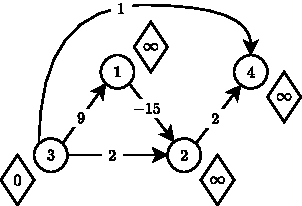
\includegraphics[width=\textwidth]{Chapter_II/DIJKSTRA-NegativeArc/a.pdf}
		\caption{}
	\end{subfigure}%
	\begin{subfigure}[b]{0.3\textwidth}
		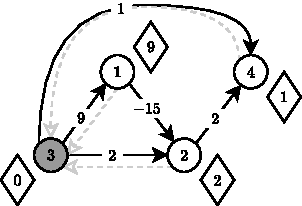
\includegraphics[width=\textwidth]{Chapter_II/DIJKSTRA-NegativeArc/b.pdf}
		\caption{}
	\end{subfigure}
	\begin{subfigure}[b]{0.3\textwidth}
		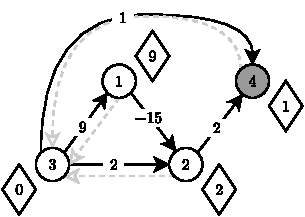
\includegraphics[width=\textwidth]{Chapter_II/DIJKSTRA-NegativeArc/c.pdf}
		\caption{}
	\end{subfigure}
	\begin{subfigure}[b]{0.3\textwidth}
		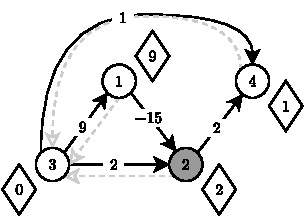
\includegraphics[width=\textwidth]{Chapter_II/DIJKSTRA-NegativeArc/d.pdf}
		\caption{}
	\end{subfigure}%
	\begin{subfigure}[b]{0.3\textwidth}
		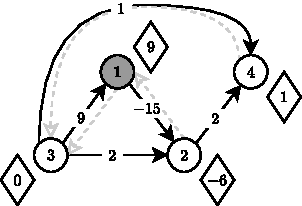
\includegraphics[width=\textwidth]{Chapter_II/DIJKSTRA-NegativeArc/e.pdf}
		\caption{}
	\end{subfigure}
	\caption{\textbf{Działanie algorytmu Dijkstry w grafie z ujemnymi kosztami krawędzi}} \label{fig:exapleDijkstraNegativArc}
\end{figure}

Jak powiedzieliśmy, algorytm Dijkstry analizuje wierzchołki grafu $G = \left( V, E \right)$ w ściśle określonym porządku tj. bada zawsze taki węzeł $v$ , którego $v.d$ jest najmniejsze spośród wszystkich pozostałych, jeszcze nie przeanalizowanych węzłów. Na kolejnych rysunkach zaznaczono kolejność przeglądania węzłów jaka wynika z tej własności (za węzeł startowy przyjmując $v_{3}$). Widzimy, że algorytm zwrócił błędną ścieżkę dla pary węzłów: $v_{3}$ i $v_{4}$ (poprawną, najkrótszą ścieżką $v_{3} \overset{*}\leadsto v_{4}$ jest ścieżka $ P = \left \langle v_{3}, v_{1}, v_{2}, v{4} \right \rangle $) ze względu na wystąpienie w grafie krawędzi o ujemnym koszcie. 
\newpage

\subsubsection{Poporawność działania}

\begin{figure}[!htbp]
	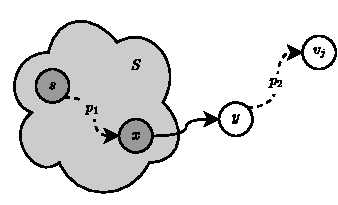
\includegraphics[width=0.3\textwidth]{Chapter_II/ProofOfDijkstra/a.pdf}
	\caption{\textbf{Dowód poprawności algorytmu Dijkstry}} Tuż przed wstawieniem wierzchołka $v_{j}$ do $S$ ten ostatni nie jest pusty. Przerywanymi strzałkami zaznaczono ścieżki $p_{1}$ oraz $p_{2}$, które mogą mieć dowolnie dużą ilość składowych (w skrajnym przypadku $s = x$ i/lub $y = v_{j}$). Dodatkowo $x \neq y$. \label{fig:proofOfDijkstra}
\end{figure}

\begin{proof}
Załóżmy indukcyjnie, że dla każdego węzła $v_{i}$ w momencie dodawania go do zbioru wierzchołków przetworzonych $S$ zachodzi $v_{i}.d = \delta \left( s, v_{i} \right)$. Pierwszy krok indukcyjny jest oczywisty, gdyż na samym początku zbiór $S$ jest pusty i założenie jest prawdziwe. Pierwszym wierzchołkiem, który jest dodawany do tego zbioru jest wierzchołek $s$, będący źródłem, którego w oczywisty sposób $s.d = 0 = \delta \left( s, s \right)$ (w grafie dla algorytmu Dijkstry założyliśmy brak krawędzi o ujemnych długościach). Przyjmijmy nie w prost, że istnieje w grafie taki wierzchołek $v_{j}$, dla którego $v_{j}.d \neq \delta \left( s, v_{j} \right)$ w trakcie jego dodawania do zbioru $S$ i będzie on pierwszym takim wierzchołkiem, jaki będziemy chcieli do tego zbioru dodać. Wiemy, że $v_{j} \neq s$ oraz, że do takiego wierzchołka na pewno istnieje najkrótsza ścieżka ze źródła $s$ (gdyby tak nie było to odpowiednio wtedy $v_{j}.d = s.d = 0 = \delta \left( s, s \right) = \delta \left( s, v_{j} \right)$ lub $v_{j}.d = \delta \left( s, v_{j} \right) = \infty $ - z własności braku ścieżki). Bezpośrednio z poprzednich spostrzeżeń wynika, że w momencie dodawania wierzchołka $v_{j}$ do zbioru $S$ ten jest niepusty i zawiera co najmniej jeden element - źródło. Niech istniejąca ścieżka z $s$ do $v_{j}$ nazywa się $P$ oraz rozważmy sytuację taką, jaką widać na rysunku \ref{fig:proofOfDijkstra}. Rozbiliśmy na nim ścieżkę $P$ na dwie składowe: $p_{1}$ i $p_{2}$, gdzie $v_{s} \overset{p_{1}}\leadsto x \overset{1}\leadsto y \overset{p_{2}}\leadsto v_{j}$ oraz pierwsza z nich składa się tylko z węzłów należących do zbioru $S$, zaś druga - tylko z węzłów poz tym zbiorem. Dodatkowo węzeł $y$ jest pierwszym na ścieżce $P$, który jest poza tym zbiorem. Pokażemy teraz, że w momencie dodawania wierzchołka $v_{j}$ ($v_{j}.d \neq \delta \left( s, v_{j} \right)$) do zbioru $S$ zachodzi $y.d = \delta \left( s, y \right)$. Aby udowodnić ten fakt, wystarczy zauważyć, że skoro wierzchołek $v_{j}$ był pierwszym takim, dla którego zachodzi $v_{j}.d \neq \delta \left( s, v_{j} \right)$, to wstawiając do zbioru $S$ wierzchołek $x$ na pewno $v_x.d = \delta \left( s, x \right)$, a ze zbieżności (lemat \ref{lem:convergenceProperty}) mamy, że zachodzi również $y.d = \delta \left( s, y \right)$ (w trakcie dodawania wierzchołka $x$ do zbioru $S$ zajdzie relaksacja krawędzi $x \overset{1}\leadsto y$, gdzie wcześniej $v_x.d = \delta \left( s, x \right)$).

Ponieważ na naszym rysunku wierzchołek $y$ występuje na ścieżce $P$ wcześniej od wierzchołka $v_{j}$ i każda krawędź w grafie ma koszt nieujemny to $ \delta \left( s, y \right) \leqslant \delta \left( s, v_{j} \right) $, co prowadzi do szeregu nierówności:

\begin{equation}
\begin{aligned}
y.d &= \delta \left( s, y \right) \\
&\leqslant \delta \left( s, v_{j} \right) \\
&\leqslant v_{j}.d \; \; \textrm{(z lematu \ref{lem:costUpperBound} o górnym ograniczeniu)}
\end{aligned}
\end{equation}

Wiemy jednak, że z własności algorytmu Dijkstry zawsze wybieramy wierzchołek spoza zbioru $S$ o jak najmniejszej wartości atrybutu $d$, a skoro oba wierzchołki ($y$ i $v_{j}$) nie należą do zbioru $S$ w chwili wyboru wierzchołka $v_{j}$ mamy zagwarantowane, że $v_{j}.d = \min \left\{ v.d : v \notin S \right\}$, w szczególności $v_{j}.d \leqslant y.d$. Dodając to ostatnie równanie do szeregu poprzednich nierówności otrzymujemy:

\begin{equation}
y.d = \delta \left( s, y \right) = \delta \left( s, v_{j} \right) = v_{j}.d
\end{equation}

Widzimy, że $ v_{j}.d = \delta \left( s, v_{j} \right) $, co jest sprzeczne z naszym założeniem (dodanie do zbioru $S$ pierwszego wierzchołka $v_{j}$ o własności  $v_{j}.d = \delta \left( s, v_{j} \right) $). Rozumowanie jest identyczne w przypadku, gdyby na ścieżkach $p_{1}$ i/lub $p_{2}$ znajdowała się dowolna liczba węzłów, spełniających nasze założenia. Pokazaliśmy zatem, że dla każdego wierzchołka $v \in V$ w momencie jego dodawania do zbioru $S$ zachodzi $v.d = \delta \left( s, v \right)$. Algorytm kończy działanie, gdy w kolejce $Q$ nie ma już żadnych wierzchołków (wszystkie zostały dodane do zbioru $S$), tak więc w momencie, gdy każdy wierzchołek spełnia $v.d = \delta \left( s, v \right)$, co kończy dowód.
\end{proof}

\section{Podstawowe struktury danych}

Jak pokazaliśmy wcześniej - efektywność algorytmu Dijkstry w głównej mierze zależy od efektywności implementacji struktury, od której będziemy wymagać wykonywania trzech, podstawowych operacji: $\textrm{\textsc{INSERT}} \left( Q, v \right)$, $\textrm{\textsc{EXTRACT-MIN}} \left( Q \right)$ i $\textrm{\textsc{DECREASE-KEY}} \left( Q, v, k \right)$. Wyspecjalizowanymi strukturami do ich wykonywania są kolejki priorytetowe, choć - jak mogliśmy się już przekonać - inne struktury, takie jak tablice, listy jednokierunkowe czy podwójnie wiązane (ang. \textit{double-linked lists}, także umożliwiają nam poprawną konstrukcję algorytmu Dijkstry. Korzystając z nich musimy jednak płacić cenę za ich wysoką nieefektywność i tak dla listy dwukierunkowej (wykorzystanej przy omawianiu algorytmu) wyszukanie najmniejszego elementu kosztuje nas proporcjonalnie do ilości wierzchołków, znajdujących się na niej w trakcie wyszukiwania. Jeżeli spojrzymy na złożoność algorytmu Dijkstry (\ref{eq:dijkstraComplexity}) natychmiastowo uzyskamy górne ograniczenie na poziomie $ O \left( \left| V \right| ^{2} \right)$, co niewiele oddala nas złożoności tak prostego algorytmu, jakim jest algorytm Bellmana-Fora.


Mówiąc o różnych wcieleniach algorytmu Dijkstry nie sposób jest więc poruszyć tematu podstawowych struktur danych, jakie możemy wykorzystać do implementacji różnych kolejek priorytetowych, ich właściwościach i czasach działania podstawowych operacji, których wykonywanie dane struktury umożliwiają - w szczególności $\textrm{\textsc{INSERT}} \left( Q, v \right)$, $\textrm{\textsc{EXTRACT-MIN}} \left( Q \right)$ i $\textrm{\textsc{DECREASE-KEY}} \left( Q, v, k \right)$. W niniejszym rozdziale omówimy takie struktury jak: kopce binarne (w uogólnionym spojrzeniu na kopce $r$-arne), kopce Fibonacciego, kolejki z przepełnieniem oraz szereg innych pomysłów, opartych o kontenery, zwane dalej kubełkami (ang. \textit{buckets}).

\section{Struktury oparte na kopcach}

Jedną ze struktur, przystosowanych do operacji charakterystycznych dla kolejki priorytetowej jest kopiec (ang. \textit{heap}). Jego najogólniejszą własnością jest to, że operacja, zwracająca najmniejszy (lub największy) element, który znajduje się w kopcu, działa w czasie stałym i polega na odwołaniu się do szczytu takiego kopca. Kopce to szczególne przypadki drzew, gdzie pomiędzy rodzicem, a potomkami zwykle jest ustalona stała relacja (w przypadku, który nas interesuje - kopiec typu \textit{min} - klucze, przechowywane przez potomków węzła $v$ powinny być zawsze większe od klucza rodzica: $v.d \leqslant v_{i} : v_{i}.\Pi = v$). Przedstawimy dwa, powszechnie znane rodzaje kopców: zwykły kopiec, do którego implementacji wykorzystamy tablicę, oraz drugi - Fibonacciego, który - jak się okaże - pomimo swojej teoretycznej przewagi w szybkości wykonywania poszczególnych operacji, w praktyce często działa wolniej od - dużo prostszego w implementacji - wspomnianej wcześniej wersji.

\subsection{Kopiec R-arny}

Kopien $R$-arny jest uogólnieniem kopca binarnego - podczas gdy dla tego drugiego każdy rodzic może posiadać do $2$ potomków, w pierwszym przypadku takich węzłów rodzic może mieć od $0$ do $R$, co zauważalnie zmniejsza wysokość takiego kopca kosztem jego szerokości. Poniższa tabelka przedstawia koszty poszczególnych operacji dla kopca binarnego i $R$-arnego:

\begin{center}
	\begin{tabular}{ccc}
		& \multicolumn{2}{c}{Kopiec} \\
		\cline{2-3}
		Operacja & binarny & $R$-arny \\
		\hline
		$\textrm{\textsc{INSERT}} \left( Q, v \right)$ & $O \left( \log \left( n \right) \right)$ & $O \left( \log_{R} \left( n \right) \right)$ \\
		$\textrm{\textsc{EXTRACT-MIN}} \left( Q \right)$ & $O \left( \log \left( n \right) \right)$ & $O \left( R \cdot \log_{R} \left( n \right) \right)$ \\
		$\textrm{\textsc{DECREASE-KEY}} \left( Q, v, k \right)$ & $O \left( \log \left( n \right) \right)$ & $O \left( \log_{R} \left( n \right) \right)$  \\
		\hline
	\end{tabular}
\end{center}

\subsubsection{Implementacja}

Algorytm wyszukiwania najkrótszych ścieżek oparty na strukturze $D$-arnego kopca jest jedynym algorytmem, który nie wymaga od nas tworzenia dodatkowych struktur. Jak dobrze wiemy, jedną z właściwości kopców jest ich zdolność do pracy w miejscu tj. nie wykorzystywania dodatkowej pamięci podczas działania. Pod pojęciem naszego grafu $G = \left( V, E \right)$ kryje się tablica $tab \left[ 1 \cdots \left| V\right| \right]$, przechowująca wierzchołki, indeksowane ich identyfikatorami ($tab[i]=v_{i}$) oraz listy sąsiedztwa, przyporządkowane do każdego z takich węzłów. Aby skorzystać z właściwości kopca, będziemy chcieli zbudować jego strukturę bezpośrednio na wspomnianej tablicy węzłów tj. kopiec o $k$ elementach będziemy chcieli przedstawić jako tablica $vertices \left[ 1 \cdots k \right]$. W takiej sytuacji, jeżeli dowolny wierzchołek $v$ znajduje się na pozycji $i <= k $ w tablicy $tab$ to znaczy, że w którymś momencie został on wstawiony do naszej kolejki priorytetowej i nie opuści jej, dopóki nie stanie się on najmniejszy spośród tych $k$ elementów. Aby jednak nie stracić informacji o pierwotnym rozmieszczeniu wierzchołków w tablicy $tab$, będziemy chcieli wprowadzić pomocniczą tablicę $heapIDArray \left[ 1 \cdots \left| V\right| \right]$, której to wartości będą odzwierciedlać faktyczne rozmieszczenie wierzchołków w $tab$ po modyfikacjach ($tab \left[ heapIDArray \left[ i \right] \right] = v_{i}$), jakich dopuści się na niej nasza kolejka priorytetowa (indeksami tablicy $tab$ pierwotnie były identyfikatory wierzchołków, a ich nie możemy zmieniać).

Zasada działania takiego kopca nie różni się niczym od zastosowania takiej samej struktury do posortowania $n$ liczb, gdzie rozmiar kopca monotonicznie rośnie w trakcie jego budowania, a następnie maleje w czasie działania takiego algorytmu. W naszym przypadku liczba jego elementów może się zwiększać jak i zmniejszać w dowolnej kolejności - jeżeli się zwiększa to ostatni element w części tablicy należącej do powiększonego kopca zamieniamy z elementem, który chcemy faktycznie do niego wstawić, a następnie "wypychamy" go ku górze (analogiczna procedura jest wykonywana podczas powiększania kopca w czasie jego budowania dla algorytmu sortowania), zaś jeżeli rozmiar kopca maleje to zachowanie, w porównaniu z algorytmem sortującym, jest identyczne.

\begin{figure}[!htbp]
	\centering
	\begin{subfigure}[b]{0.33\textwidth}
		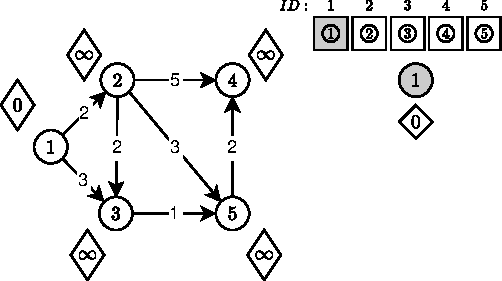
\includegraphics[width=\textwidth]{Chapter_II/R-HEAP-Example/a.pdf}
		\caption{}
	\end{subfigure}%
	\begin{subfigure}[b]{0.33\textwidth}
		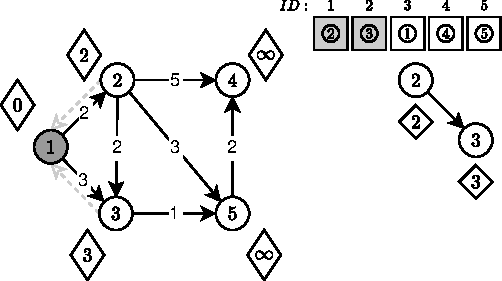
\includegraphics[width=\textwidth]{Chapter_II/R-HEAP-Example/b.pdf}
		\caption{}
	\end{subfigure}
	\begin{subfigure}[b]{0.33\textwidth}
		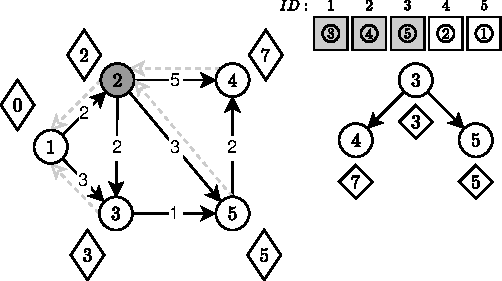
\includegraphics[width=\textwidth]{Chapter_II/R-HEAP-Example/c.pdf}
		\caption{}
	\end{subfigure}
	\begin{subfigure}[b]{0.33\textwidth}
		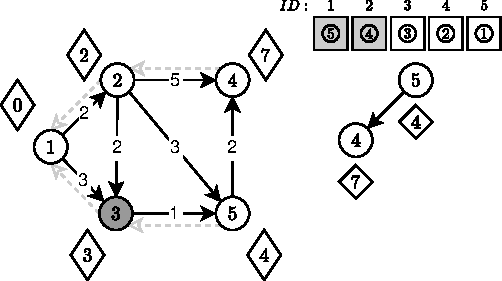
\includegraphics[width=\textwidth]{Chapter_II/R-HEAP-Example/d.pdf}
		\caption{}
	\end{subfigure}%
	\begin{subfigure}[b]{0.33\textwidth}
		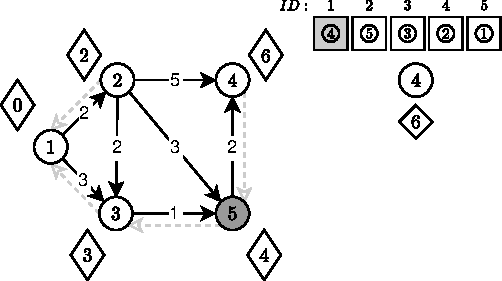
\includegraphics[width=\textwidth]{Chapter_II/R-HEAP-Example/e.pdf}
		\caption{}
	\end{subfigure}
	\begin{subfigure}[b]{0.33\textwidth}
		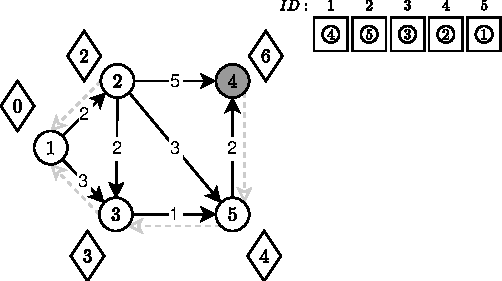
\includegraphics[width=\textwidth]{Chapter_II/R-HEAP-Example/f.pdf}
		\caption{}
	\end{subfigure}
	\caption{\textbf{Działanie algorytmu Dijkstry w oparciu o kopiec $R$-arny} \textbf{(a)} Sytuacja po zainicjowaniu grafu $G$ przez \textsf{INIT-GRAH} ze źródłem $v_{1}$. W tablicy na szaro zaznaczone są elementy należące do kopca, przedstawionego poniżej. Niech $k$ oznacza rozmiar kopca, tablica $tab$ jest indeksowana od $1$. \textbf{(b)} Z kopca zostaje usunięty węzeł $v_{1}$ ($k=0$). W wyniku relaksacji na kopiec zostaje przeniesiony węzeł $v_{2}$ ($k=1$ i $tab \left[ k \right] = v_{2}$), zaś na stare miejsce wstawionego węzła zostaje przeniesiony węzeł $v_{1}$. Analogicznie na koniec kopca wstawiany jest $v_{3}$  ($k=2$, $tab \left[ k \right] = v_{3}$) w wyniku czego $tab \left[ 3 \right] = v_{1}$. \textbf{(c)} Z kopca zostaje pobrany węzeł $v_{2}$, a na szczyt stosu zostaje przeniesiony ostatni element w kopcu ($v_{3}$). W wyniku relaksacji krawędzi, wychodzących w pobranego węzła, do kopca zostają dodane węzły: $v_{4}$ i $v_{5}$. Tablica $tab$ zmienia się odpowiednio: $\left\{ 3 \right\} \left[ 2 \right]  \left[ 1 \right]  \left[ 4 \right]  \left[ 5 \right] \rightarrow \left\{ 3 \right\} \left\{ 4 \right\}  \left[ 1 \right]  \left[ 2 \right]  \left[ 5 \right] \rightarrow \left\{ 3 \right\} \left\{ 4 \right\}  \left\{ 5 \right\}  \left[ 2 \right]  \left[ 1 \right]$, gdzie w klamrach "$\left\{\right\}$"~ zostały zaznaczone węzły, znajdujące się w kopcu. Żadna operacja nie narusza własności kopca. \textbf{(d)} Wybrano kolejny węzeł ze szczytu stosu: $v_{3}$, zamieniając go z ostatnim elementem w kopcu i zmniejszając jego rozmiar ($k=2$). Zachowana jest własność kopca. W wyniku relaksacji zostają zmienione atrybuty: $v_{5}.\Pi = v_{3}$ i $v_{5}.d = 4$. \textbf{(e-f)} Z kopca zostaje zabrany jego najmniejszy element: $v_{5}$ i wykonywana jest operacja \textsf{RELAX} dla krawędzi z niego wychodzących. Na szczyt kopca zostaje wstawiony jego ostatni element ($k=1$). Własność kopca jest zachowana.} \label{fig:exampleDHeap}
\end{figure}

\subsubsection{Złożoność obliczeniowa}

Uzupełniając wzór \ref{eq:dijkstraComplexity} na ogólną złożoność generycznego algorytmu Dijkstry z wykorzystaniem kolejek priorytetowych dla kopców $R$-arnych natychmiast otrzymujemy $O \left( m \cdot \log_{d} \left( n \right) + n \cdot \left[ \log_{d} \left( n \right) + d \cdot \log_{d} \left( n \right) \right] \right) = O \left( m \cdot \log_{d} \left( n \right) + n \cdot d \cdot \log_{d} \left( n \right) \right) $ (dla przejrzystości zapisu przyjęliśmy $ n = \left| V\right|$ i $ m = \left| E \right|$). Dla kopca binarnego mamy: $O \left( m \cdot \log \left( n \right) + n \cdot \log \left( n \right) \right) = O \left( m \cdot \log \left( n \right) \right) $ dla $m \geqslant n $ (stałe wyeliminowaliśmy). Przypomnijmy sobie, że naiwna implementacja algorytmu Dijkstry miała złożoność $ O \left( m + n^{2} \right) = O \left( n^{2} \right)$. Łatwo zauważyć, że dla bardzo gęstych grafów (gdzie $ m = \Omega \left( n^{2} \right) $) nasz nowy algorytm asymptotycznie staje się wolniejszy nawet od wspomnianej, naiwnej implementacji, jednak sytuacja zmienia się na korzyść kopców, gdy ilość krawędzi w grafie jest z góry ograniczona przez $ O \left( \frac{n^{2}}{ \log \left( n \right) } \right)$ ( wtedy $ O \left( m \cdot \log \left( n \right) \right) \leqslant O \left( \frac{n^{2}}{\log \left( n \right)} \cdot \log \left( n \right) \right) = O \left( n^{2} \right)$).

Z kolei dla kopców, których arność jest większa ($d \geqslant 2$) mamy: $O \left( m \cdot \log_{d} \left( n \right) + n \cdot d \cdot \log_{d} \left( n \right) \right) $. Z tego bezpośrednio wynika, że optymalną wartością parametru $d$ jest $ \max \left\{ 2, \left \lceil \frac{m}{n} \right \rceil \right\} $, dla którego zrównują nam się obie strony sumy, otrzymanej wcześniej, złożoności ($ n \cdot \frac{m}{n} \cdot \log_{d} \left( n \right) = m \cdot \log_{d} \left( n \right) $). Otrzymaliśmy złożoność algorytmu Dijkstry, opartego o kopce $R$-arne, który znów w zależności od sieci, dla której go zastosujemy, będzie porównywalny albo do podstawowej, naiwnej implementacji tego samego algorytmu ( dla sieci gęstych, gdzie $ m = \Omega \left( n^{2} \right)$ mamy: $O \left( m \cdot \log_{d} \left( n \right) \right) = O \left( n^{2} \cdot \log_{\frac{n^{2}}{n}} \left( n \right) \right) = O \left( n^{2} \cdot \log_{n} \left( n \right) \right) = O \left( n^{2} \right)$), albo do opartego na kopcu binarnym (w przypadku, gdy sieć jest bardzo rzadka). Dla tej drugiej możliwości otrzymujemy natychmiastowo złożoność $O \left( n \cdot \log \left( n \right) \right)$ dla $m = \O \left( n \right)$.

Co więcej, jeżeli założymy $m = \Omega \left( n^{1+\epsilon} \right)$ dla $\epsilon > 0$ i $d = \left \lceil \frac{m}{n} \right \rceil > 2$ to będziemy mogli wyprowadzić następujący ciąg równości:

\begin{equation}
	\begin{aligned}
		O \left( m \cdot \log_{d} \left( n \right) \right) &= O \left( m \cdot \frac{\log \left( n \right)}{\log \left( d \right)} \right) \; \; \left( \textrm{zamiana podstawy logarytmu} \right) \\
		&= O \left( m \cdot \frac{\log \left( n \right)}{\log \left( n^{\epsilon} \right)} \right) \; \; \left( d = \left \lceil \frac{m}{n} \right \rceil = \frac{n^{1+\epsilon}}{n} \right) \\
		&= O \left( m \cdot \frac{\log \left( n \right)}{ \epsilon \cdot \log \left( n \right)} \right) \; \; \left( \log_{a} \left( b^{c} \right) = c \cdot \log_{a} \left( b \right) \right) \\
		&= O \left( \frac{m}{\epsilon} \right) \\
		&= O \left( m \right) \; \; \left( \frac{1}{\epsilon} \textrm{jest stałą.} \right)
	\end{aligned}
\end{equation}


Jeśli $\epsilon = 1$ to $ m = \Omega \left( n^{2} \right)$, a ten wariant analizowaliśmy już wcześniej. Widzimy więc, że w zależności od gęstości grafu te same algorytmy mogą zachowywać się zupełnie inaczej, a co za tym idzie - nie jesteśmy w stanie wskazać jednej implementacji algorytmu wyszukiwania najkrótszych ścieżek, która działałaby równie szybko (w porównaniu do reszty algorytmów) dla każdej z możliwych sieci.

\subsubsection{Drzewa}

Strukturami bardzo podobnymi do kopców są drzewa $K$-arne - należy wręcz powiedzieć, że kopce są \textbf{pełnymi drzewami} (ang. \textit{complete tree}), podczas gdy struktura zwykłego drzewa jest mniej rygorystyczna. Pełnym drzewem $R$-arnym (jakim jest kopiec tej samej arności) nazywamy takie drzewo, na poziomach którego, poza ostatnim, wszystkie węzły mają dokładnie $R$ potomków. W przypadku drzew $K$-arnych każdy węzeł może mieć co najwyżej $K$ węzłów potomnych, co nie musi wcale oznaczać, że stworzone tak drzewo, jest drzewem pełnym. Obie struktury da się zaimplementować przy wykorzystaniu zwykłych tablic choć, w przypadku drzew, pomiędzy kolejnymi elementami takie tablicy mogą pojawić się miejsca puste, gdy któryś z węzłów drzewa ma mniej niż $K$ potomków. Inne są także założenia samych struktur: każdy węzeł w drzewie $K$-arnym posiada tyleż potomków w ściśle zdefiniowanym porządku (niemalejącym lub nierosnącym), zaś reguły, odnoszące się do kopców nic o takim porządku nie mówią - jedyna własność, która musi zostać spełniona dla węzła to przewyższanie jego priorytetem wszystkich swoich potomków (bądź posiadanie najmniejszego priorytetu pośród nich w przypadku kopca typu \textit{min}). Bezpośrednią konsekwencją tych własności są różne zastosowania wymienionych struktur danych: 

\begin{center}
	\begin{savenotes}
		\begin{tabular}{ccccc}
			& \multicolumn{2}{c}{Drzewo} & \multicolumn{2}{c}{Kopciec} \\
			\cline{2-5}
			Operacja & binarne\footnote{Przedstawiono czasy dla odpowiednio: drzew zbalansowanych (takich jak RBT, AVL) i drzew niezbalansowanych, dla których pesymistyczna wysokość wynosi $O \left( n\right)$.} & $K$-arne & binarny & $R$-arny \\
			\hline
			$\textrm{\textsc{INSERT}} \left( Q, v \right)$ & $ O \left( \log \left( n \right) \right)$ / $ O \left( 1 \right) $ & $O \left( K \cdot \log_{K} \left( n \right) \right)$ & $O \left( \log \left( n \right) \right)$ & $O \left( \log_{R} \left( n \right) \right)$ \\
			$\textrm{\textsc{EXTRACT-MIN}} \left( Q \right)$ & $ O \left( \log \left( n \right) \right)$  / $ O \left( n \right) $ & $ O \left( \log_{K} \left( n\right) \right)$ & $O \left( \log \left( n \right) \right)$ & $O \left( R \cdot \log_{R} \left( n \right) \right)$ \\
			$\textrm{\textsc{DECREASE-KEY}} \left( Q, v, k \right)$ & $ O \left( \log \left( n \right) \right)$  / $ O \left( 1 \right) $ & $O \left( K \cdot \log_{K} \left( n \right) \right)$ & $O \left( \log \left( n \right) \right)$ & $O \left( \log_{R} \left( n \right) \right)$  \\
			$\textrm{\textsc{SEARCH}} \left( Q, k \right)$ & $ O \left( \log \left( n \right) \right)$ / $ O \left( n \right) $ & $O \left( K \cdot \log_{K} \left( n \right) \right)$ & $O \left( n \right)$ & $ O \left( n \right) $  \\
			\hline
		\end{tabular}
	\end{savenotes}
\end{center}

strukturę drzew stosuje się dla problemów, gdzie nacisk jest kładziony na wyszukiwanie elementów po ich właściwościach, zaś wybieranie minimum jest sprawą drugorzędną. Odwrotna sytuacja występuje w przypadku kopców, które w żaden sposób nie wspierają operacji wyszukiwania, sprowadzając ją do przeszukania całej tablicy reprezentującej kopiec. Innymi słowy: drzewa $K$-arne nie są przystosowane do pełnienia roli kolejki priorytetowej. Przywołując wzór na ogólną złożoność algorytmu Dijkstry ( \ref{eq:dijkstraComplexity} ):

\begin{equation}
O \left( m \cdot O \left( \textrm{\textsc{DK}} \left( Q, v, k \right) \right) + n \cdot \left[ O \left( \textrm{\textsc{I}} \left( Q, v \right) \right) + O \left( \textrm{\textsc{EM}} \left( Q \right) \right) \right] \right)
\end{equation}\label{eq:dijkstraComplexityShort}

i porównując czasy wykonywanych operacji dojdziemy do następujących złożoności:

\begin{itemize}
\item $ O \left( \left( n + m \right) \cdot \log \left( n \right) \right)$  dla zbalansowanych drzew przeszukiwań binarnych,
\item $ O \left( m + n^{2} \right) = O \left( n^{2} \right) $ dla niezbalansowanych drzew przeszukiwań binarnych,
\item $ O \left( \left( n + m \right) \cdot K \cdot \log_{K} \left( n \right) \right)$  dla zbalansowanych drzew $K$-arnych,
\end{itemize}

gdzie złożoności algorytmu wyszukiwania najkrótszych ścieżek w oparciu o kopce policzyliśmy w poprzednim podrozdziale i wynosiły one: $ O \left( \left( n + m \right) \cdot \log \left( n \right) \right) $ i $ O \left( m \cdot \log_{d} \left( n \right) \right) $ odpowiednio dla kopców binarnych i $R$-arnych. Na podstawie powyższego zestawienia możemy podejrzewać, że struktura zbalansowanych drzew binarnych jest w pewnym stopniu konkurencyjna dla kopców tej samej arności \footnote{Jeżeli byśmy chcieli uzyskać dla zbalansowanych drzew $K$-arnych takie samo oszacowanie na asymptotyczną złożoność obliczeniową, musielibyśmy przyjąć $d = \frac{m}{m+n}$ (wtedy $O \left( \left( n + m \right) \cdot K \cdot \log_{K} \left( n \right) \right) = O \left( m \cdot \log_{K} \left( n \right) \right) $), lecz nie możemy mieć struktury, której współczynnik rozgałęzienia ($d$) jest mniejszy od dwóch (przypadek drzewa binarnego)}, jednak w tej analizie nie braliśmy w ogóle pod uwagę stałych czynników, jakie pojawiają się podczas wykonywania wszystkich, wyżej przeanalizowanych, operacji, a które przemawiają na niekorzyść zbalansowanych drzew przeszukiwań - te struktury (takie jak Drzewo Czerwono-Czarne czy Adelsona-Velskiego-Landisa) są znacznie bardziej złożone przez co wymagają nie tylko więcej pamięci na przechowywanie danych, ale też wykazują się mniejszą efektywnością niż prostsze struktury o tych samych, asymptotycznych czasach działania. Jak się przekonamy w następnym rozdziale, prawidłowość ta dotyczy również kopców Fibonacciego, które, pomimo lepszych wyników teoretycznych, nie sprawdzą się jako kolejka priorytetowa dla algorytmu Dijkstry właśnie ze względu na możliwość zastąpienia tej struktury przez dużo prostsze i mniej skomplikowane rozwiązania.

\subsection{Kopiec Fibonacciego}

Przedstawiona w tym rozdziale implementacja algorytmu Dijkstry jako kolejkę priorytetową będzie wykorzystywać jedną z bardziej złożonych struktur danych, jakie będziemy omawiać - kopce Fibonacciego. Zaletą jej wykorzystania okaże się amortyzacyjnie lepszy czas wykonywania dla dwóch, podstawowych operacji, wykorzystywanych podczas działania naszego algorytmu - $\textrm{\textsc{INSERT}} \left( Q, v \right)$ i $\textrm{\textsc{DECREASE-KEY}} \left( Q, v, k \right)$.


Dodatkowo, aby jeszcze przyśpieszyć działanie podstawowej wersji implementacji kopca Fibonacciego, możemy dostosować ją do właściwego środowiska, w którym to oparta na kopcu kolejka priorytetowa będzie wykorzystywana. Pierwszą rzeczą, jaką możemy zauważyć to sposób zmiany ilości elementów, które znajdują się na kopcu - w odróżnieniu od algorytmu wyszukiwania najkrótszych ścieżek dla danego grafu $ G = \left( V, E \right)$, gdzie ilość węzłów jest z góry znana, dla ogólnego przypadku nie jesteśmy w stanie nic powiedzieć o maksymalnej ilości elementów, jakie znajdą się na kopcu. Konsekwencją tej niewiedzy jest konieczność rezerwowania dodatkowej pamięci dla pomocniczych tablic za każdym razem, gdy wykonujemy operację $\textrm{\textsc{EXTRACT-MIN}} \left( Q \right)$. Choć rozmiar takich tablic jest z góry znany i wynosi on $ \left \lfloor \log_{\Phi} \left( n \right) \right \rfloor $ to bez znajomości maksymalnej wartości parametru $n$ nie jesteśmy w stanie tego faktu w jakikolwiek sposób wykorzystać. Inaczej jest w przypadku, gdy mamy dany graf $G$, którego liczba wierzchołków wynosi dokładnie $ \left| V \right|$, co przekłada się na maksymalną liczbę elementów, jakie jednocześnie mogą znaleźć się na kopcu Fibonacciego - wówczas z każdą operacją $\textrm{\textsc{EXTRACT-MIN}} \left( Q \right)$ korzystamy z tej samej tablicy pomocniczej $A \left[ 1 \cdots \left \lfloor \log_{\Phi} \left( n \right) \right \rfloor \right]$, którą "czyścimy" pod sam koniec procedury, budując - zgodnie z podstawowym algorytmem - nową listę korzeni kopca Fibonacciego (iterując po całej tablicy i dodając, trzymane w niej drzewa ukorzenione, do głównej listy, zaś elementy samej tablicy zerując). Inną, bardziej oczywistą modyfikacją, jest wykorzystanie faktu, iż każda lista, która znajduje się w wewnętrznej strukturze kopca, jest cykliczną listą dwukierunkową co, znów w przypadku wykonywania procedury $\textrm{\textsc{EXTRACT-MIN}} \left( Q \right)$, pozwoli nam zaoszczędzić trochę czasu podczas pierwszych kroków tego algorytmu (zamiast usuwać najmniejszy element $v$ z listy korzeni i iteracyjnie przepinać potomków tego węzła do wspomnianej listy, możemy "rozerwać" obie listy w wybranym przez nas punkcie, a następnie połączyć w czasie $O \left( 1 \right)$, zaś usuwanie powiązań między potomkami usuwanego węzła tymczasowo zignorować - podstawowa wersja algorytmu podczas przepinania węzłów $u$ takich, że $ u.\Pi = v$ ustawia te parametry na wartość \KwNull. Podkreślić należy słowo: "tymczasowo"~, gdyż ta czynność zostanie wykonana w momencie rekonstrukcji kopca Fibonacciego z drzew, przechowywanych w tablicy $A \left[ 1 \cdots \left \lfloor \log_{\Phi} \left( n \right) \right \rfloor \right]$ - wiedząc, że każdy jej element przechowuje wskaźnik do przyszłego węzła na liście korzeni będziemy dla każdego elementu z tablicy $A$ dodatkowo niszczyć wskazanie tego węzła na jego rodzica, którego nie zniszczyliśmy wcześniej.).

\begin{figure}[!htbp]
	\centering
	\begin{subfigure}[b]{0.45\textwidth}
		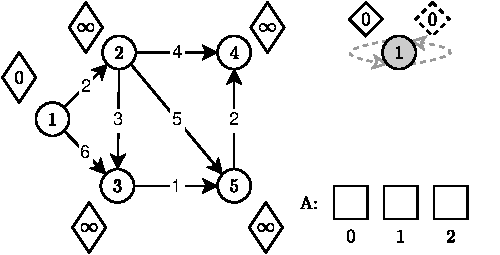
\includegraphics[width=\textwidth]{Chapter_II/FIBONACCI-Example/a.pdf}
		\caption{}
	\end{subfigure}%
	\begin{subfigure}[b]{0.45\textwidth}
		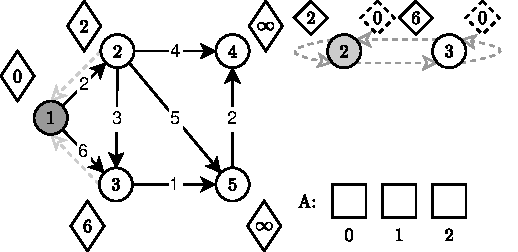
\includegraphics[width=\textwidth]{Chapter_II/FIBONACCI-Example/b.pdf}
		\caption{}
	\end{subfigure}
	\begin{subfigure}[b]{0.45\textwidth}
		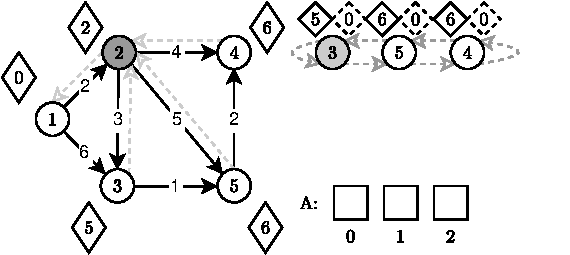
\includegraphics[width=\textwidth]{Chapter_II/FIBONACCI-Example/c.pdf}
		\caption{}
	\end{subfigure}%
	\begin{subfigure}[b]{0.45\textwidth}
		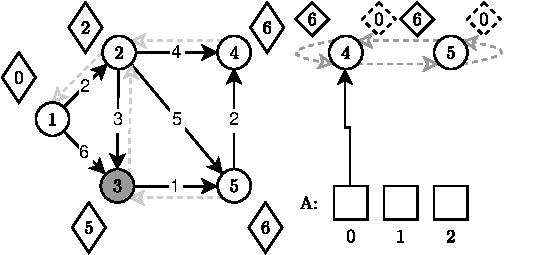
\includegraphics[width=\textwidth]{Chapter_II/FIBONACCI-Example/d.pdf}
		\caption{}
	\end{subfigure}
	\begin{subfigure}[b]{0.45\textwidth}
		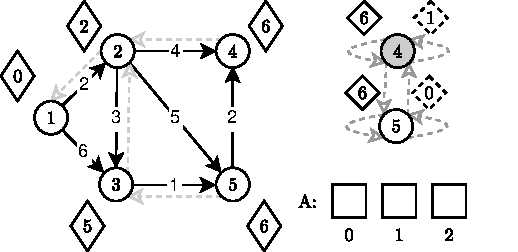
\includegraphics[width=\textwidth]{Chapter_II/FIBONACCI-Example/e.pdf}
		\caption{}
	\end{subfigure}%
	\begin{subfigure}[b]{0.45\textwidth}
		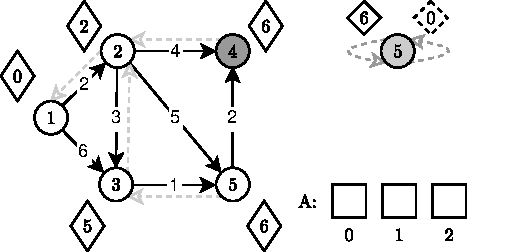
\includegraphics[width=\textwidth]{Chapter_II/FIBONACCI-Example/f.pdf}
		\caption{}
	\end{subfigure}
	\caption{\textbf{Działanie algorytmu Dijkstry w oparciu o kopiec Fibonacciego}} \textbf{(a)} \textbf{(b)} \textbf{(c)} \textbf{(d)} \textbf{(e)} \textbf{(f)} \label{fig:exampleFibonacci}
\end{figure}

\section{Struktury oparte na kubełkach}
\label{sec:dijkstraBuckets}

nC+1 kubełków, nic ciekawego

brak rysunku, bo za duży

%\Blindtext

\subsection{Z przepełnieniem}

%\Blindtext

budujemy a < C + 1 main bucketów i overflow. każdy main bucket ma szerokość 1. Ogólnie main: $[a(i),a(i)+a-1]$. Skanujemy main buckety i wykonujemy relaksacje, dorzucając do mainów lub overflow. Gdy dojdziemy do końca maina to aktualizujemy ich szerokość $a(i) = min_overflow$ i przenosimy z overflowu do main wszystkie [a(i),a(i)+a-1] i reskanujemy mainy od 0 do a. Jeśli przeskanowaliśmy wszystkie i overflow pusty to koniec.

\begin{figure}[!htbp]
	\centering
	\begin{subfigure}[b]{0.33\textwidth}
		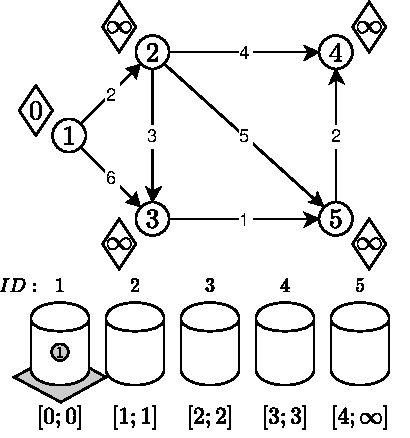
\includegraphics[width=\textwidth]{Chapter_II/1/a.pdf}
		\caption{}
	\end{subfigure}%
	\begin{subfigure}[b]{0.33\textwidth}
		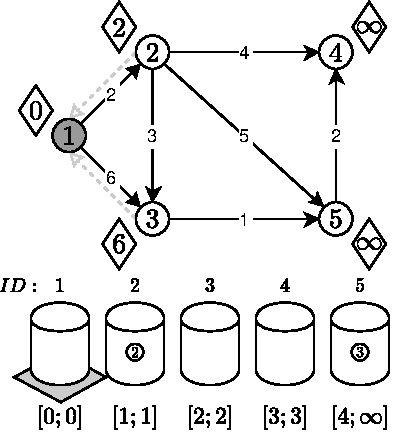
\includegraphics[width=\textwidth]{Chapter_II/1/b.pdf}
		\caption{}
	\end{subfigure}
	\begin{subfigure}[b]{0.33\textwidth}
		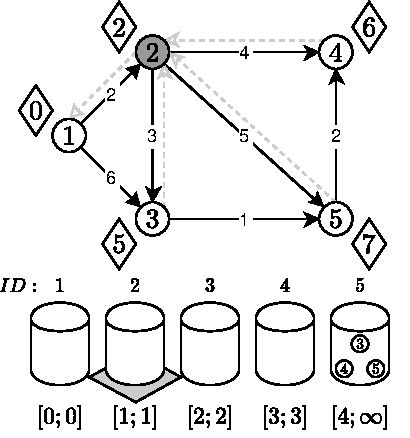
\includegraphics[width=\textwidth]{Chapter_II/1/c.pdf}
		\caption{}
	\end{subfigure}
	\begin{subfigure}[b]{0.33\textwidth}
		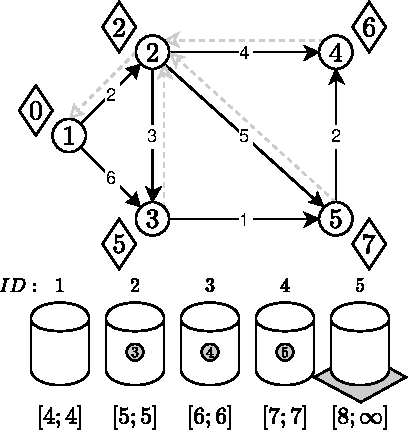
\includegraphics[width=\textwidth]{Chapter_II/1/d.pdf}
		\caption{}
	\end{subfigure}%
	\begin{subfigure}[b]{0.33\textwidth}
		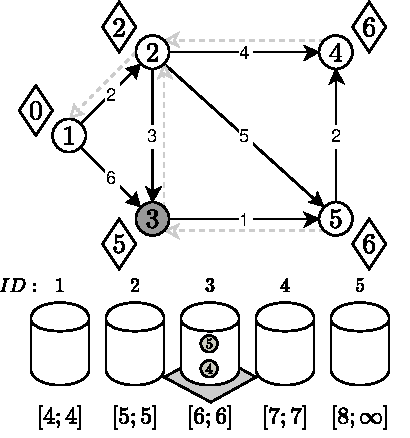
\includegraphics[width=\textwidth]{Chapter_II/1/e.pdf}
		\caption{}
	\end{subfigure}
	\begin{subfigure}[b]{0.33\textwidth}
		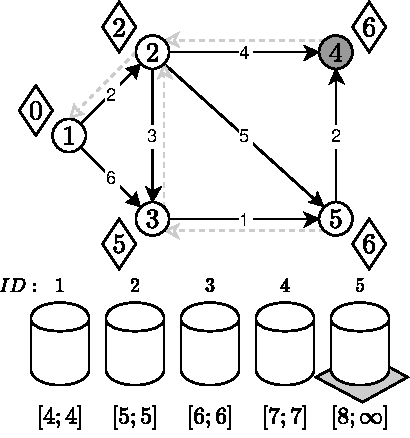
\includegraphics[width=\textwidth]{Chapter_II/1/f.pdf}
		\caption{}
	\end{subfigure}
	\caption{\textbf{Działanie algorytmu Bellmana-Forda} \textbf{(a)} Sytuacja po zainicjowaniu grafu $G = \left( V, E \right)$ przez \textsf{INIT-GRAPH} ze źródłem $v_{s}.id = 1$. \textbf{(b)} Warunek $ v.d > u.d + c_{uv} $ dla krawędzi $ \left( u, v \right) $ spełniony jest tylko dla krawędzi: $ \left( 1, 2 \right) $ i $ \left( 1, 3 \right) $ i dla tych węzłów ( $v_{2}$ i $v_{3}$ ) zostały zaktualizowani ich poprzednicy (zaznaczeni szarymi strzałkami) oraz etykiety $d$. Dla pozostałych algorytm nie wprowadził żadnych zmian w trakcie iterowania po wszystkich $ A \left( i \right) : i \in \left\{ 1, \ldots, 5\right\}$. \textbf{(c)} Przyjęliśmy kolejność iterowania po wszystkich łukach (pętla $3-4$) zgodną z kolejnością ponumerowania węzłów na rysunkach. Przyjmijmy ponadto rosnącą kolejność identyfikatorów węzłów, do której łuki prowadzą tj. podczas drugiej iteracji algorytm wykonuje operację \textsf{RELAX} na krawędziach w kolejności: $ \left( 1, 2 \right) $, $ \left( 1, 3 \right) $ (dla których relaksacja nie wprowadzi żadnych zmian), $ \left( 2, 3 \right) $ (zostaje zaktualizowany węzeł $v_{3}$ - jego wartość $d$ przyjmie długość odnalezionej, krótszej ścieżki oraz otrzyma nowego rodzica), $ \left( 2, 4 \right) $, $ \left( 2, 5 \right) $, \textbf{(d)} $ \left( 3, 5 \right) $ i $ \left( 5, 2 \right) $. Dla normalnej wersji algorytmu powinniśmy wykonać jeszcze 3 iteracje po wszystkich krawędziach, jednak wprowadziliśmy modyfikację, która przerywa działanie algorytmu, jeżeli podczas pełnej iteracji nie nastąpi w grafie $G$ żadna zmiana.} \label{fig:exampleBellmanFord}
\end{figure}

\subsection{Dial}

%\Blindtext

skanujemy wszystkie kubełki w kółko. C+1 kubełków

\begin{figure}[!htbp]
	\centering
	\begin{subfigure}[b]{0.33\textwidth}
		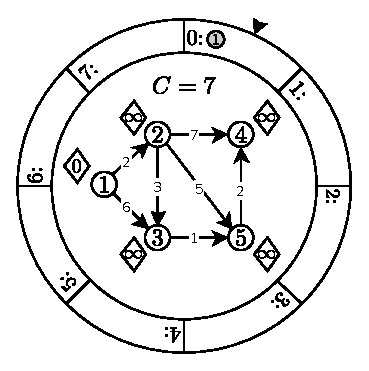
\includegraphics[width=\textwidth]{Chapter_II/2/a.eps}
		\caption{}
	\end{subfigure}%
	\begin{subfigure}[b]{0.33\textwidth}
		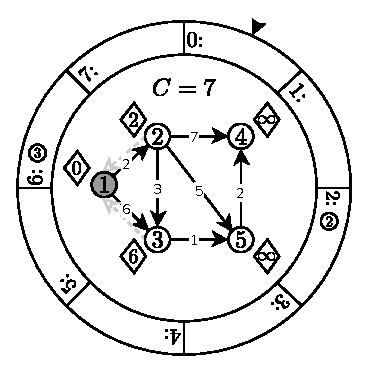
\includegraphics[width=\textwidth]{Chapter_II/2/b.eps}
		\caption{}
	\end{subfigure}
	\begin{subfigure}[b]{0.33\textwidth}
		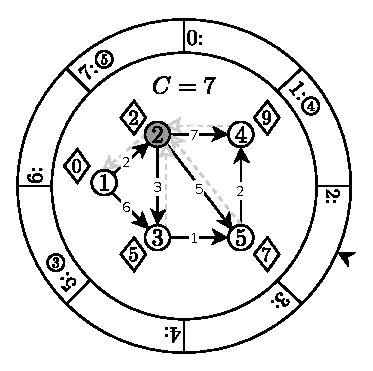
\includegraphics[width=\textwidth]{Chapter_II/2/c.eps}
		\caption{}
	\end{subfigure}
	\begin{subfigure}[b]{0.33\textwidth}
		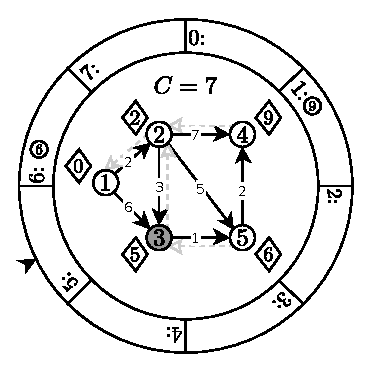
\includegraphics[width=\textwidth]{Chapter_II/2/d.eps}
		\caption{}
	\end{subfigure}%
	\begin{subfigure}[b]{0.33\textwidth}
		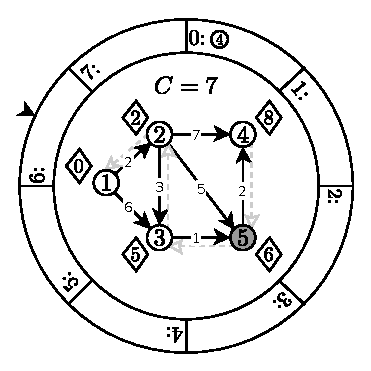
\includegraphics[width=\textwidth]{Chapter_II/2/e.eps}
		\caption{}
	\end{subfigure}
	\begin{subfigure}[b]{0.33\textwidth}
		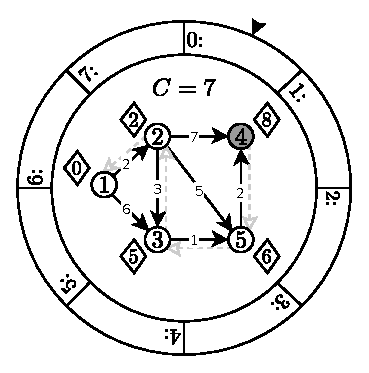
\includegraphics[width=\textwidth]{Chapter_II/2/f.eps}
		\caption{}
	\end{subfigure}
	\caption{\textbf{Działanie algorytmu Bellmana-Forda} \textbf{(a)} Sytuacja po zainicjowaniu grafu $G = \left( V, E \right)$ przez \textsf{INIT-GRAPH} ze źródłem $v_{s}.id = 1$. \textbf{(b)} Warunek $ v.d > u.d + c_{uv} $ dla krawędzi $ \left( u, v \right) $ spełniony jest tylko dla krawędzi: $ \left( 1, 2 \right) $ i $ \left( 1, 3 \right) $ i dla tych węzłów ( $v_{2}$ i $v_{3}$ ) zostały zaktualizowani ich poprzednicy (zaznaczeni szarymi strzałkami) oraz etykiety $d$. Dla pozostałych algorytm nie wprowadził żadnych zmian w trakcie iterowania po wszystkich $ A \left( i \right) : i \in \left\{ 1, \ldots, 5\right\}$. \textbf{(c)} Przyjęliśmy kolejność iterowania po wszystkich łukach (pętla $3-4$) zgodną z kolejnością ponumerowania węzłów na rysunkach. Przyjmijmy ponadto rosnącą kolejność identyfikatorów węzłów, do której łuki prowadzą tj. podczas drugiej iteracji algorytm wykonuje operację \textsf{RELAX} na krawędziach w kolejności: $ \left( 1, 2 \right) $, $ \left( 1, 3 \right) $ (dla których relaksacja nie wprowadzi żadnych zmian), $ \left( 2, 3 \right) $ (zostaje zaktualizowany węzeł $v_{3}$ - jego wartość $d$ przyjmie długość odnalezionej, krótszej ścieżki oraz otrzyma nowego rodzica), $ \left( 2, 4 \right) $, $ \left( 2, 5 \right) $, \textbf{(d)} $ \left( 3, 5 \right) $ i $ \left( 5, 2 \right) $. Dla normalnej wersji algorytmu powinniśmy wykonać jeszcze 3 iteracje po wszystkich krawędziach, jednak wprowadziliśmy modyfikację, która przerywa działanie algorytmu, jeżeli podczas pełnej iteracji nie nastąpi w grafie $G$ żadna zmiana.} \label{fig:exampleBellmanFord}
\end{figure}

\subsection{Aproksymacja zakresu}

%\Blindtext

skanujemy po kolei wszystkie kubełki, każdy z nich ma kolejkę fifo z wierzchołkami

W najgorszym przypadku by doskanować się do najmniejszego elementu musimy przeglądnąć wszystkie C+1 kubełków i wybrać z fifo ogon. Dodawanie/przepinanie wierzchołków wymaga wrzucenia nodea na szczyt listy fifo i zrzucenia go do pozycji, gdzie niżej jest już węzeł o <= koszcie.
W najgorszym przypadku czeka nas m updatów, każdy trwający b (wsadzanie do listy, by był zachowany priorytet) - szerokość kubełka (lecz czemu zakładamy, że na liście jest max b elementów??).
\begin{figure}[!htbp]
	\centering
	\begin{subfigure}[b]{0.33\textwidth}
		\includegraphics[width=\textwidth]{Chapter_II/3/a.eps}
		\caption{}
	\end{subfigure}%
	\begin{subfigure}[b]{0.33\textwidth}
		\includegraphics[width=\textwidth]{Chapter_II/3/b.eps}
		\caption{}
	\end{subfigure}
	\begin{subfigure}[b]{0.33\textwidth}
		\includegraphics[width=\textwidth]{Chapter_II/3/c.eps}
		\caption{}
	\end{subfigure}
	\begin{subfigure}[b]{0.33\textwidth}
		\includegraphics[width=\textwidth]{Chapter_II/3/d.eps}
		\caption{}
	\end{subfigure}%
	\begin{subfigure}[b]{0.33\textwidth}
		\includegraphics[width=\textwidth]{Chapter_II/3/e.eps}
		\caption{}
	\end{subfigure}
	\begin{subfigure}[b]{0.33\textwidth}
		\includegraphics[width=\textwidth]{Chapter_II/3/f.eps}
		\caption{}
	\end{subfigure}
	\caption{\textbf{Działanie algorytmu Bellmana-Forda} \textbf{(a)} Sytuacja po zainicjowaniu grafu $G = \left( V, E \right)$ przez \textsf{INIT-GRAPH} ze źródłem $v_{s}.id = 1$. \textbf{(b)} Warunek $ v.d > u.d + c_{uv} $ dla krawędzi $ \left( u, v \right) $ spełniony jest tylko dla krawędzi: $ \left( 1, 2 \right) $ i $ \left( 1, 3 \right) $ i dla tych węzłów ( $v_{2}$ i $v_{3}$ ) zostały zaktualizowani ich poprzednicy (zaznaczeni szarymi strzałkami) oraz etykiety $d$. Dla pozostałych algorytm nie wprowadził żadnych zmian w trakcie iterowania po wszystkich $ A \left( i \right) : i \in \left\{ 1, \ldots, 5\right\}$. \textbf{(c)} Przyjęliśmy kolejność iterowania po wszystkich łukach (pętla $3-4$) zgodną z kolejnością ponumerowania węzłów na rysunkach. Przyjmijmy ponadto rosnącą kolejność identyfikatorów węzłów, do której łuki prowadzą tj. podczas drugiej iteracji algorytm wykonuje operację \textsf{RELAX} na krawędziach w kolejności: $ \left( 1, 2 \right) $, $ \left( 1, 3 \right) $ (dla których relaksacja nie wprowadzi żadnych zmian), $ \left( 2, 3 \right) $ (zostaje zaktualizowany węzeł $v_{3}$ - jego wartość $d$ przyjmie długość odnalezionej, krótszej ścieżki oraz otrzyma nowego rodzica), $ \left( 2, 4 \right) $, $ \left( 2, 5 \right) $, \textbf{(d)} $ \left( 3, 5 \right) $ i $ \left( 5, 2 \right) $. Dla normalnej wersji algorytmu powinniśmy wykonać jeszcze 3 iteracje po wszystkich krawędziach, jednak wprowadziliśmy modyfikację, która przerywa działanie algorytmu, jeżeli podczas pełnej iteracji nie nastąpi w grafie $G$ żadna zmiana.} \label{fig:exampleBellmanFord}
\end{figure}

\subsection{Kubełki wielopoziomowe}

Mamy k kubełków niskiego poziomu, każdy o szerokości 1. Mamy floor(n*C/k) + 1 kubełków wysokiego poziomu, każdy szerokości [k*i,k*(i+1)-1] dla każdego i. Np. dla n=7, C=2 i k = 5 mamy 3 wysokich (0..2) i ostatni ma [10,14]. Dla ceil(nC/k) i nC=15 i k = 5 mamy też 0..2 i jest źle.

Skanujemy po kolei wysokie, przerzucając z każdego po kolei do niskiego poziomu. Skanujemy niski poziom, gdy jest już pusty, to idziemy do następnego wysokiego. Przenosimy z niego do niskich. I tak dalej.

\begin{figure}[!htbp]
	\centering
	\begin{subfigure}[b]{0.45\textwidth}
		\includegraphics[width=\textwidth]{Chapter_II/4/a.pdf}
		\caption{}
	\end{subfigure}%
	\qquad
	\begin{subfigure}[b]{0.45\textwidth}
		\includegraphics[width=\textwidth]{Chapter_II/4/b.pdf}
		\caption{}
	\end{subfigure}
	\begin{subfigure}[b]{0.45\textwidth}
		\includegraphics[width=\textwidth]{Chapter_II/4/c.pdf}
		\caption{}
	\end{subfigure}
	\qquad
	\begin{subfigure}[b]{0.45\textwidth}
		\includegraphics[width=\textwidth]{Chapter_II/4/d.pdf}
		\caption{}
	\end{subfigure}%
	\caption{\textbf{Działanie algorytmu Bellmana-Forda} \textbf{(a)} Sytuacja po zainicjowaniu grafu $G = \left( V, E \right)$ przez \textsf{INIT-GRAPH} ze źródłem $v_{s}.id = 1$. \textbf{(b)} Warunek $ v.d > u.d + c_{uv} $ dla krawędzi $ \left( u, v \right) $ spełniony jest tylko dla krawędzi: $ \left( 1, 2 \right) $ i $ \left( 1, 3 \right) $ i dla tych węzłów ( $v_{2}$ i $v_{3}$ ) zostały zaktualizowani ich poprzednicy (zaznaczeni szarymi strzałkami) oraz etykiety $d$. Dla pozostałych algorytm nie wprowadził żadnych zmian w trakcie iterowania po wszystkich $ A \left( i \right) : i \in \left\{ 1, \ldots, 5\right\}$. \textbf{(c)} Przyjęliśmy kolejność iterowania po wszystkich łukach (pętla $3-4$) zgodną z kolejnością ponumerowania węzłów na rysunkach. Przyjmijmy ponadto rosnącą kolejność identyfikatorów węzłów, do której łuki prowadzą tj. podczas drugiej iteracji algorytm wykonuje operację \textsf{RELAX} na krawędziach w kolejności: $ \left( 1, 2 \right) $, $ \left( 1, 3 \right) $ (dla których relaksacja nie wprowadzi żadnych zmian), $ \left( 2, 3 \right) $ (zostaje zaktualizowany węzeł $v_{3}$ - jego wartość $d$ przyjmie długość odnalezionej, krótszej ścieżki oraz otrzyma nowego rodzica), $ \left( 2, 4 \right) $, $ \left( 2, 5 \right) $, \textbf{(d)} $ \left( 3, 5 \right) $ i $ \left( 5, 2 \right) $. Dla normalnej wersji algorytmu powinniśmy wykonać jeszcze 3 iteracje po wszystkich krawędziach, jednak wprowadziliśmy modyfikację, która przerywa działanie algorytmu, jeżeli podczas pełnej iteracji nie nastąpi w grafie $G$ żadna zmiana.} \label{fig:exampleBellmanFord}
\end{figure}
	
\begin{figure}[!htbp]
	\ContinuedFloat
	\centering
	\begin{subfigure}[b]{0.45\textwidth}
		\includegraphics[width=\textwidth]{Chapter_II/4/e.pdf}
		\caption{}
	\end{subfigure}%
	\qquad
	\begin{subfigure}[b]{0.45\textwidth}
		\includegraphics[width=\textwidth]{Chapter_II/4/f.pdf}
		\caption{}
	\end{subfigure}
	\begin{subfigure}[b]{0.45\textwidth}
		\includegraphics[width=\textwidth]{Chapter_II/4/g.pdf}
		\caption{}
	\end{subfigure}
	\qquad
	\begin{subfigure}[b]{0.45\textwidth}
		\includegraphics[width=\textwidth]{Chapter_II/4/h.pdf}
		\caption{}
	\end{subfigure}%
	\caption{\textbf{Działanie algorytmu Bellmana-Forda} \textbf{(a)} Sytuacja po zainicjowaniu grafu $G = \left( V, E \right)$ przez \textsf{INIT-GRAPH} ze źródłem $v_{s}.id = 1$. \textbf{(b)} Warunek $ v.d > u.d + c_{uv} $ dla krawędzi $ \left( u, v \right) $ spełniony jest tylko dla krawędzi: $ \left( 1, 2 \right) $ i $ \left( 1, 3 \right) $ i dla tych węzłów ( $v_{2}$ i $v_{3}$ ) zostały zaktualizowani ich poprzednicy (zaznaczeni szarymi strzałkami) oraz etykiety $d$. Dla pozostałych algorytm nie wprowadził żadnych zmian w trakcie iterowania po wszystkich $ A \left( i \right) : i \in \left\{ 1, \ldots, 5\right\}$. \textbf{(c)} Przyjęliśmy kolejność iterowania po wszystkich łukach (pętla $3-4$) zgodną z kolejnością ponumerowania węzłów na rysunkach. Przyjmijmy ponadto rosnącą kolejność identyfikatorów węzłów, do której łuki prowadzą tj. podczas drugiej iteracji algorytm wykonuje operację \textsf{RELAX} na krawędziach w kolejności: $ \left( 1, 2 \right) $, $ \left( 1, 3 \right) $ (dla których relaksacja nie wprowadzi żadnych zmian), $ \left( 2, 3 \right) $ (zostaje zaktualizowany węzeł $v_{3}$ - jego wartość $d$ przyjmie długość odnalezionej, krótszej ścieżki oraz otrzyma nowego rodzica), $ \left( 2, 4 \right) $, $ \left( 2, 5 \right) $, \textbf{(d)} $ \left( 3, 5 \right) $ i $ \left( 5, 2 \right) $. Dla normalnej wersji algorytmu powinniśmy wykonać jeszcze 3 iteracje po wszystkich krawędziach, jednak wprowadziliśmy modyfikację, która przerywa działanie algorytmu, jeżeli podczas pełnej iteracji nie nastąpi w grafie $G$ żadna zmiana.} \label{fig:exampleBellmanFord}
\end{figure}

%\Blindtext

\subsection{Kopce pozycyjne}

\subsubsection{nC}

Mamy n*C kubełków (floor(log2(numberOfNodes)+log2(maxCost)) + 2 dokładnie), gdzie każdy zbiera nody o dystansie:
$
[0] = [min+0;min+0]
[1] = [min+2^(i-1);min+2^i-1] = [min+1;min+1]
[2] = ...
[n*c] [... ; <= n*C]$

Skanujemy je po kolei i jeśli ma długość = [k;k] albo jest tylko 1 node to wyciągamy nody z kubełka i robimy normalną relaksację (przed tym wyciągamy minimalny element - jeśli [k;k] lub to wyciągamy pierwszy lepszy, jeśli nie to przyda nam się to dalej). Jeśli w buckecie jest więcej węzłów o różnych etykietach to mamy już wyciągnięte minimum - min będzie się równać etykiecie tego minimalnego węzła, a pozostałe od 0 do j (gdzie badamy j'ty kubełek) będą zmienione, zachowując swoje pojemności (tylko min się zmieni, a pojemności trzymamy w tablicy osobno). J'ty kubełek zostanie zmieniony o +1, tak, aby j-1 miał [...;u[j]-1], [u[j];u[j]], a następny miał już naturalnie u[j]+1 - czyli teraz będzie się stykać. Realocujemy potem wszystkie węzły z j'tego kubełka do niższych. Ich nowych kubełków szukamy od j do 0, gdyż 1) od wyższych jest lepiej, bo mają większe zakresy i większa szansa, że się szybko zatrzymamy, 2) możemy mieć węzeł, który nawet po realokacji zostanie w j'tym kubełku.


\begin{figure}[!htbp]
	\centering
	\begin{subfigure}[b]{0.3\textwidth}
		\includegraphics[width=\textwidth]{Chapter_II/7/a.pdf}
		\caption{}
	\end{subfigure}
	\begin{subfigure}[b]{0.3\textwidth}
		\includegraphics[width=\textwidth]{Chapter_II/7/b.pdf}
		\caption{}
	\end{subfigure}
	\begin{subfigure}[b]{0.3\textwidth}
		\includegraphics[width=\textwidth]{Chapter_II/7/c.pdf}
		\caption{}
	\end{subfigure}
	\begin{subfigure}[b]{0.3\textwidth}
		\includegraphics[width=\textwidth]{Chapter_II/7/d.pdf}
		\caption{}
	\end{subfigure}
	\begin{subfigure}[b]{0.3\textwidth}
		\includegraphics[width=\textwidth]{Chapter_II/7/e.pdf}
		\caption{}
	\end{subfigure}
	\begin{subfigure}[b]{0.3\textwidth}
		\includegraphics[width=\textwidth]{Chapter_II/7/f.pdf}
		\caption{}
	\end{subfigure}
	\caption{\textbf{Działanie algorytmu Bellmana-Forda} \textbf{(a)} Sytuacja po zainicjowaniu grafu $G = \left( V, E \right)$ przez \textsf{INIT-GRAPH} ze źródłem $v_{s}.id = 1$. \textbf{(b)} Warunek $ v.d > u.d + c_{uv} $ dla krawędzi $ \left( u, v \right) $ spełniony jest tylko dla krawędzi: $ \left( 1, 2 \right) $ i $ \left( 1, 3 \right) $ i dla tych węzłów ( $v_{2}$ i $v_{3}$ ) zostały zaktualizowani ich poprzednicy (zaznaczeni szarymi strzałkami) oraz etykiety $d$. Dla pozostałych algorytm nie wprowadził żadnych zmian w trakcie iterowania po wszystkich $ A \left( i \right) : i \in \left\{ 1, \ldots, 5\right\}$. \textbf{(c)} Przyjęliśmy kolejność iterowania po wszystkich łukach (pętla $3-4$) zgodną z kolejnością ponumerowania węzłów na rysunkach. Przyjmijmy ponadto rosnącą kolejność identyfikatorów węzłów, do której łuki prowadzą tj. podczas drugiej iteracji algorytm wykonuje operację \textsf{RELAX} na krawędziach w kolejności: $ \left( 1, 2 \right) $, $ \left( 1, 3 \right) $ (dla których relaksacja nie wprowadzi żadnych zmian), $ \left( 2, 3 \right) $ (zostaje zaktualizowany węzeł $v_{3}$ - jego wartość $d$ przyjmie długość odnalezionej, krótszej ścieżki oraz otrzyma nowego rodzica), $ \left( 2, 4 \right) $, $ \left( 2, 5 \right) $, \textbf{(d)} $ \left( 3, 5 \right) $ i $ \left( 5, 2 \right) $. Dla normalnej wersji algorytmu powinniśmy wykonać jeszcze 3 iteracje po wszystkich krawędziach, jednak wprowadziliśmy modyfikację, która przerywa działanie algorytmu, jeżeli podczas pełnej iteracji nie nastąpi w grafie $G$ żadna zmiana.} \label{fig:exampleBellmanFord}
\end{figure}

\subsubsection{C}

Mamy C+1 kubełków (ceil(log2(maxCost+1)) + 2 dokładnie), gdzie każdy zbiera nody o dystansie:

$[0] = [min+0;min+0]
[1] = [min+2^(i-1);min+2^i-1] = [min+1;min+1]
[2] = ...
[c] [... ; ...]$

a ostatni zbiera wszystko ponad. Ide jest taka, by miał n*C jako max i u[c]+1 jako minimum, lecz chcemy uniknąć problemu z poprzedniej implementacji: dla n*C dla największych testów ( 23947347 węzłów i 58333344 połączeń) liczba n*C była aż 51 bitowa, co nakładało konieczność użycia takowych w całym algorytmie, zwiększając potrzebną pamięć ( same łuki to 26 bitów). Tutaj umowa taka, że overflow to kubełek widmo, który definiujemy inaczej (podobnie jak w alg. z faktycznym overflowem).

Skanujemy je po kolei i jeśli ma długość = [k;k] albo jest tylko 1 node to wyciągamy nody z kubełka i robimy normalną relaksację, JEŚLI bucket to nie jest overflow - z niego z definicji tylko robimy realokacje. (przed tym wyciągamy minimalny element - jeśli [k;k] lub to wyciągamy pierwszy lepszy, jeśli nie to przyda nam się to dalej - TU ZMIANA w odniesieniu do porzedniego - wyciągamy już konkretny element w środku if'a lub elsa, co oszczędza 1 if'a, a kolejność zbudowania warunku jest taka, by były sprawdzane warunki od najczęściej występującego, do najrzadziej - jeśli nie overflow I (nie jest i < 2 - kubełek na pewno długości 1 LUB inny kubełek długości 1 LUB gdybyśmy wyciągnęli z listy 2 kierunkowej to nie byłoby już w niej elementów)). Jeśli robimy zwykła relaksację to ZMIANA: robimy ją tylko gdy bucket toNode jest overflowem ( DOMYŚLNIE KAŻDY NOWY JEST W NIM) I ALBO nie był wcześniej wykorzystywany ALBO w przeciwnym wypadku, jeśli jego nowy dystans jest mniejszy od minimum overflowu. Inaczej nie ma sensu robić update'a. Tak samo dla toNode gdy jest z niższych bucketów - także aktualizujemy końcówkę overflowu ( jeśli będziemy robić for'a to jeśli node ma trafić do overflowu- czyli ma większą etykietę niż początek overflowu - to MUSIMY dociągnąć drugi "]" tak, aby nowa etykieta wstawianego noda się mieściła pomiędzy). Ta końcówka nie ma nigdzie więcej znaczenia, bo korzystamy z niej tylko tutaj. TO, że coś jest w overflow to NIE ZNACZY, że nie było używane (mogło zostać w overflow). Jeśli nie został spełniony żaden z warunków (!= NULL i dystans nie jest mniejszy od obecnego bucketa) to nie robimy fora ZMIANA, a jeśli któryś był spełniony to na pewno nowy bucket będzie mniejszy od starego lub == NULL - nie był wykorzystywany.

 Jeśli w buckecie jest więcej węzłów o różnych etykietach to ZMIANA wyciągamy dopiero minimum - min będzie się równać etykiecie tego minimalnego węzła, a pozostałe od 0 do j (gdzie badamy j'ty kubełek) będą zmienione, zachowując swoje pojemności (tylko min się zmieni, a pojemności trzymamy w tablicy osobno). J'ty kubełek zostanie zmieniony na [max;max]. Realocujemy potem wszystkie węzły z j'tego kubełka do niższych. Ich nowych kubełków szukamy od j do 0, gdyż 1) od wyższych jest lepiej, bo mają większe zakresy i większa szansa, że się szybko zatrzymamy, 2) możemy mieć węzeł, który nawet po realokacji zostanie w j'tym kubełku.
 
 JEŚLI skanowany bucket to overflow to nie ma ograniczeń min(..., maxRange) dla nowych zasięgów bucketów (gdyż overflow z definicji był nieskończony), czyli prawie tak jakbyśmy zaczynali od początku, tyle, że przesunięci o min. MaxRange ustawiamy tylko, gdy skanujemy niżej niż overflow - wtedy = ->end z bucketa, który skanujemy. Potem usawiamy J'ty [max;max] oraz ustawiamy ->begin overflowa, jeśli trzeba na o 1 większy niż poprzedzający go kubełek - jeśli zmienialiśmy rozmiar tego ostatniego.
 
 Przy realocacji także patrzymy, czy zmiana zakresów spowoduje zmiany bucketów nodów, które są w tym j'tym buckecie i były przyczyną przeskalowania bucketów od 0 do j - zostawienie [max;max] spowoduje, że nie przesuniemy niepotrzebnie tych węzłów, które były na końcu tego kubełka. Reszte przesuwamy w dół.
%\Blindtext



\begin{figure}[!htbp]
	\centering
	\begin{subfigure}[b]{0.3\textwidth}
		\includegraphics[width=\textwidth]{Chapter_II/8/a.pdf}
		\caption{}
	\end{subfigure}
	\begin{subfigure}[b]{0.3\textwidth}
		\includegraphics[width=\textwidth]{Chapter_II/8/b.pdf}
		\caption{}
	\end{subfigure}
	\begin{subfigure}[b]{0.3\textwidth}
		\includegraphics[width=\textwidth]{Chapter_II/8/c.pdf}
		\caption{}
	\end{subfigure}
	\begin{subfigure}[b]{0.3\textwidth}
		\includegraphics[width=\textwidth]{Chapter_II/8/d.pdf}
		\caption{}
	\end{subfigure}
	\begin{subfigure}[b]{0.3\textwidth}
		\includegraphics[width=\textwidth]{Chapter_II/8/e.pdf}
		\caption{}
	\end{subfigure}
	\begin{subfigure}[b]{0.3\textwidth}
		\includegraphics[width=\textwidth]{Chapter_II/8/f.pdf}
		\caption{}
	\end{subfigure}
	\caption{\textbf{Działanie algorytmu Bellmana-Forda} \textbf{(a)} Sytuacja po zainicjowaniu grafu $G = \left( V, E \right)$ przez \textsf{INIT-GRAPH} ze źródłem $v_{s}.id = 1$. \textbf{(b)} Warunek $ v.d > u.d + c_{uv} $ dla krawędzi $ \left( u, v \right) $ spełniony jest tylko dla krawędzi: $ \left( 1, 2 \right) $ i $ \left( 1, 3 \right) $ i dla tych węzłów ( $v_{2}$ i $v_{3}$ ) zostały zaktualizowani ich poprzednicy (zaznaczeni szarymi strzałkami) oraz etykiety $d$. Dla pozostałych algorytm nie wprowadził żadnych zmian w trakcie iterowania po wszystkich $ A \left( i \right) : i \in \left\{ 1, \ldots, 5\right\}$. \textbf{(c)} Przyjęliśmy kolejność iterowania po wszystkich łukach (pętla $3-4$) zgodną z kolejnością ponumerowania węzłów na rysunkach. Przyjmijmy ponadto rosnącą kolejność identyfikatorów węzłów, do której łuki prowadzą tj. podczas drugiej iteracji algorytm wykonuje operację \textsf{RELAX} na krawędziach w kolejności: $ \left( 1, 2 \right) $, $ \left( 1, 3 \right) $ (dla których relaksacja nie wprowadzi żadnych zmian), $ \left( 2, 3 \right) $ (zostaje zaktualizowany węzeł $v_{3}$ - jego wartość $d$ przyjmie długość odnalezionej, krótszej ścieżki oraz otrzyma nowego rodzica), $ \left( 2, 4 \right) $, $ \left( 2, 5 \right) $, \textbf{(d)} $ \left( 3, 5 \right) $ i $ \left( 5, 2 \right) $. Dla normalnej wersji algorytmu powinniśmy wykonać jeszcze 3 iteracje po wszystkich krawędziach, jednak wprowadziliśmy modyfikację, która przerywa działanie algorytmu, jeżeli podczas pełnej iteracji nie nastąpi w grafie $G$ żadna zmiana.} \label{fig:exampleBellmanFord}
\end{figure}

\section{Analiza}

%\Blindtext
%\Blindtext